\documentclass[11pt]{article}
% =======================================================================
%   Shared style for CS 300 notes.
%   Usage: place `% =======================================================================
%   Shared style for CS 300 notes.
%   Usage: place `% =======================================================================
%   Shared style for CS 300 notes.
%   Usage: place `\input{../../notes-style.tex}` right after \documentclass
%   in each chapter's lectures.tex and notes.tex.
% =======================================================================

% ---- Layout -----------------------------------------------------------
\usepackage[margin=1in]{geometry}
\usepackage{parskip}        % space between paragraphs, no indent
\usepackage{microtype}      % subtle kerning/spacing improvements

% ---- Colors (muted palette, easy on light-sensitive eyes) -------------
\usepackage{xcolor}
\definecolor{pagebg}       {HTML}{FAF6F0}  % warm cream background
\definecolor{bodyfg}       {HTML}{3D3A36}  % warm dark gray body text
\definecolor{heading}      {HTML}{3D6A6B}  % muted teal
\definecolor{subheading}   {HTML}{5B7A9C}  % dusty blue
\definecolor{accent}       {HTML}{8A6B4A}  % warm tan
\definecolor{linkcol}      {HTML}{5B7A9C}  % same as subheading
\definecolor{mutedtext}    {HTML}{6B6560}  % secondary / caption text
\definecolor{rulecol}      {HTML}{C8BFB0}  % separator / rule

% Callout box palette
\definecolor{defnFrame}    {HTML}{9DB89B}  \definecolor{defnBack}    {HTML}{EEF2E8}
\definecolor{ideaFrame}    {HTML}{9FB4CD}  \definecolor{ideaBack}    {HTML}{E8EEF5}
\definecolor{warnFrame}    {HTML}{CFAE87}  \definecolor{warnBack}    {HTML}{F5EDDF}
\definecolor{noteFrame}    {HTML}{BFA6AE}  \definecolor{noteBack}    {HTML}{F2E8EE}
\definecolor{exFrame}      {HTML}{9FBDBD}  \definecolor{exBack}      {HTML}{E8F0F0}
\definecolor{codeBack}     {HTML}{F3EDE2}
\definecolor{codeBorder}   {HTML}{D4CBBA}
\definecolor{codeKeyword}  {HTML}{6B4F7A}
\definecolor{codeString}   {HTML}{8A6B4A}
\definecolor{codeComment}  {HTML}{8A857F}

% ---- Page background + base text color --------------------------------
\usepackage{pagecolor}
\pagecolor{pagebg}
\color{bodyfg}

% ---- Fonts ------------------------------------------------------------
\usepackage[T1]{fontenc}
\IfFileExists{libertine.sty}{%
    \usepackage{libertine}      % warm, readable serif
    \usepackage[scaled=0.95]{inconsolata}  % softer monospace
}{}

% ---- Hyperref ---------------------------------------------------------
\usepackage{hyperref}
\hypersetup{
    colorlinks=true,
    linkcolor=linkcol,
    urlcolor=linkcol,
    citecolor=linkcol,
    pdfborder={0 0 0},
}

% ---- Section styling --------------------------------------------------
\usepackage[explicit]{titlesec}
\titleformat{\section}
    {\color{heading}\Large\bfseries}
    {\color{heading}\thesection\hspace{0.6em}}{0pt}{#1}
\titleformat{\subsection}
    {\color{subheading}\large\bfseries}
    {\color{subheading}\thesubsection\hspace{0.5em}}{0pt}{#1}
\titleformat{\subsubsection}
    {\color{accent}\normalsize\bfseries}
    {\color{accent}\thesubsubsection\hspace{0.5em}}{0pt}{#1}
\titleformat{\paragraph}[runin]
    {\color{accent}\bfseries}{}{0pt}{#1.}

\titlespacing*{\section}{0pt}{1.6em}{0.6em}
\titlespacing*{\subsection}{0pt}{1.2em}{0.4em}

% ---- Enumerate / itemize spacing --------------------------------------
\usepackage{enumitem}
\setlist[itemize]{leftmargin=1.4em, itemsep=2pt, topsep=4pt}
\setlist[enumerate]{leftmargin=1.6em, itemsep=2pt, topsep=4pt}

% ---- Code listings ----------------------------------------------------
\usepackage{listings}
\lstdefinestyle{notescode}{
    backgroundcolor=\color{codeBack},
    basicstyle=\ttfamily\small\color{bodyfg},
    keywordstyle=\color{codeKeyword}\bfseries,
    stringstyle=\color{codeString},
    commentstyle=\color{codeComment}\itshape,
    frame=single,
    framesep=6pt,
    rulecolor=\color{codeBorder},
    showstringspaces=false,
    breaklines=true,
    xleftmargin=10pt,
    xrightmargin=10pt,
    aboveskip=8pt,
    belowskip=8pt,
}
\lstset{style=notescode}

% ---- Callout boxes (tcolorbox) ----------------------------------------
\usepackage[most]{tcolorbox}

\newtcolorbox{defnbox}[1][]{
    enhanced, breakable,
    colback=defnBack, colframe=defnFrame, coltitle=bodyfg,
    title={\bfseries Definition \textemdash\ #1},
    fonttitle=\bfseries,
    boxrule=0.5pt, arc=2pt, left=8pt, right=8pt, top=6pt, bottom=6pt,
    attach boxed title to top left={xshift=10pt, yshift=-6pt},
    boxed title style={colback=defnFrame, colframe=defnFrame, arc=2pt},
    before skip=8pt, after skip=8pt,
}
\newtcolorbox{ideabox}[1][]{
    enhanced, breakable,
    colback=ideaBack, colframe=ideaFrame, coltitle=bodyfg,
    title={\bfseries Key idea #1},
    boxrule=0.5pt, arc=2pt, left=8pt, right=8pt, top=6pt, bottom=6pt,
    attach boxed title to top left={xshift=10pt, yshift=-6pt},
    boxed title style={colback=ideaFrame, colframe=ideaFrame, arc=2pt},
    before skip=8pt, after skip=8pt,
}
\newtcolorbox{warnbox}[1][]{
    enhanced, breakable,
    colback=warnBack, colframe=warnFrame, coltitle=bodyfg,
    title={\bfseries Gotcha #1},
    boxrule=0.5pt, arc=2pt, left=8pt, right=8pt, top=6pt, bottom=6pt,
    attach boxed title to top left={xshift=10pt, yshift=-6pt},
    boxed title style={colback=warnFrame, colframe=warnFrame, arc=2pt},
    before skip=8pt, after skip=8pt,
}
\newtcolorbox{notebox}[1][]{
    enhanced, breakable,
    colback=noteBack, colframe=noteFrame, coltitle=bodyfg,
    title={\bfseries Aside #1},
    boxrule=0.5pt, arc=2pt, left=8pt, right=8pt, top=6pt, bottom=6pt,
    attach boxed title to top left={xshift=10pt, yshift=-6pt},
    boxed title style={colback=noteFrame, colframe=noteFrame, arc=2pt},
    before skip=8pt, after skip=8pt,
}
\newtcolorbox{examplebox}[1][]{
    enhanced, breakable,
    colback=exBack, colframe=exFrame, coltitle=bodyfg,
    title={\bfseries Example #1},
    boxrule=0.5pt, arc=2pt, left=8pt, right=8pt, top=6pt, bottom=6pt,
    attach boxed title to top left={xshift=10pt, yshift=-6pt},
    boxed title style={colback=exFrame, colframe=exFrame, arc=2pt},
    before skip=8pt, after skip=8pt,
}

% ---- TikZ graph styles (added 2026-04-25 for ch_10 augmentation) ------
% tcolorbox[most] already loads tikz; this block declares the libraries
% + shared `vertex` / `edge` styles used by ch_10's general directed-graph
% diagrams. ch_9's tree-style TikZ uses inline overrides and is
% unaffected. Simple circle nodes + arrow edges only -- no production
% styling.
\usetikzlibrary{arrows.meta, positioning, calc}
\tikzset{
    vertex/.style={circle, draw, minimum size=7mm, inner sep=0pt,
                   font=\small, thick},
    vsource/.style={vertex, fill=ideaBack},
    vdone/.style={vertex, fill=defnBack},
    edge/.style={->, >=Stealth, thick},
    uedge/.style={-, thick},
    treeedge/.style={->, >=Stealth, thick},
    backedge/.style={->, >=Stealth, thick, dashed, red!70!black},
    fwdedge/.style={->, >=Stealth, thick, blue!60!black},
    crossedge/.style={->, >=Stealth, thick, green!50!black, dotted},
    mstedge/.style={-, very thick, accent},
}

% ---- Title block ------------------------------------------------------
\usepackage{titling}
\pretitle{\begin{center}\color{heading}\LARGE\bfseries}
\posttitle{\end{center}\vskip -0.4em}
\preauthor{\begin{center}\color{mutedtext}\normalsize}
\postauthor{\end{center}}
\predate{\begin{center}\color{mutedtext}\small}
\postdate{\end{center}\vspace{0.4em}{\color{rulecol}\hrule height 0.4pt}\vspace{1.2em}}
` right after \documentclass
%   in each chapter's lectures.tex and notes.tex.
% =======================================================================

% ---- Layout -----------------------------------------------------------
\usepackage[margin=1in]{geometry}
\usepackage{parskip}        % space between paragraphs, no indent
\usepackage{microtype}      % subtle kerning/spacing improvements

% ---- Colors (muted palette, easy on light-sensitive eyes) -------------
\usepackage{xcolor}
\definecolor{pagebg}       {HTML}{FAF6F0}  % warm cream background
\definecolor{bodyfg}       {HTML}{3D3A36}  % warm dark gray body text
\definecolor{heading}      {HTML}{3D6A6B}  % muted teal
\definecolor{subheading}   {HTML}{5B7A9C}  % dusty blue
\definecolor{accent}       {HTML}{8A6B4A}  % warm tan
\definecolor{linkcol}      {HTML}{5B7A9C}  % same as subheading
\definecolor{mutedtext}    {HTML}{6B6560}  % secondary / caption text
\definecolor{rulecol}      {HTML}{C8BFB0}  % separator / rule

% Callout box palette
\definecolor{defnFrame}    {HTML}{9DB89B}  \definecolor{defnBack}    {HTML}{EEF2E8}
\definecolor{ideaFrame}    {HTML}{9FB4CD}  \definecolor{ideaBack}    {HTML}{E8EEF5}
\definecolor{warnFrame}    {HTML}{CFAE87}  \definecolor{warnBack}    {HTML}{F5EDDF}
\definecolor{noteFrame}    {HTML}{BFA6AE}  \definecolor{noteBack}    {HTML}{F2E8EE}
\definecolor{exFrame}      {HTML}{9FBDBD}  \definecolor{exBack}      {HTML}{E8F0F0}
\definecolor{codeBack}     {HTML}{F3EDE2}
\definecolor{codeBorder}   {HTML}{D4CBBA}
\definecolor{codeKeyword}  {HTML}{6B4F7A}
\definecolor{codeString}   {HTML}{8A6B4A}
\definecolor{codeComment}  {HTML}{8A857F}

% ---- Page background + base text color --------------------------------
\usepackage{pagecolor}
\pagecolor{pagebg}
\color{bodyfg}

% ---- Fonts ------------------------------------------------------------
\usepackage[T1]{fontenc}
\IfFileExists{libertine.sty}{%
    \usepackage{libertine}      % warm, readable serif
    \usepackage[scaled=0.95]{inconsolata}  % softer monospace
}{}

% ---- Hyperref ---------------------------------------------------------
\usepackage{hyperref}
\hypersetup{
    colorlinks=true,
    linkcolor=linkcol,
    urlcolor=linkcol,
    citecolor=linkcol,
    pdfborder={0 0 0},
}

% ---- Section styling --------------------------------------------------
\usepackage[explicit]{titlesec}
\titleformat{\section}
    {\color{heading}\Large\bfseries}
    {\color{heading}\thesection\hspace{0.6em}}{0pt}{#1}
\titleformat{\subsection}
    {\color{subheading}\large\bfseries}
    {\color{subheading}\thesubsection\hspace{0.5em}}{0pt}{#1}
\titleformat{\subsubsection}
    {\color{accent}\normalsize\bfseries}
    {\color{accent}\thesubsubsection\hspace{0.5em}}{0pt}{#1}
\titleformat{\paragraph}[runin]
    {\color{accent}\bfseries}{}{0pt}{#1.}

\titlespacing*{\section}{0pt}{1.6em}{0.6em}
\titlespacing*{\subsection}{0pt}{1.2em}{0.4em}

% ---- Enumerate / itemize spacing --------------------------------------
\usepackage{enumitem}
\setlist[itemize]{leftmargin=1.4em, itemsep=2pt, topsep=4pt}
\setlist[enumerate]{leftmargin=1.6em, itemsep=2pt, topsep=4pt}

% ---- Code listings ----------------------------------------------------
\usepackage{listings}
\lstdefinestyle{notescode}{
    backgroundcolor=\color{codeBack},
    basicstyle=\ttfamily\small\color{bodyfg},
    keywordstyle=\color{codeKeyword}\bfseries,
    stringstyle=\color{codeString},
    commentstyle=\color{codeComment}\itshape,
    frame=single,
    framesep=6pt,
    rulecolor=\color{codeBorder},
    showstringspaces=false,
    breaklines=true,
    xleftmargin=10pt,
    xrightmargin=10pt,
    aboveskip=8pt,
    belowskip=8pt,
}
\lstset{style=notescode}

% ---- Callout boxes (tcolorbox) ----------------------------------------
\usepackage[most]{tcolorbox}

\newtcolorbox{defnbox}[1][]{
    enhanced, breakable,
    colback=defnBack, colframe=defnFrame, coltitle=bodyfg,
    title={\bfseries Definition \textemdash\ #1},
    fonttitle=\bfseries,
    boxrule=0.5pt, arc=2pt, left=8pt, right=8pt, top=6pt, bottom=6pt,
    attach boxed title to top left={xshift=10pt, yshift=-6pt},
    boxed title style={colback=defnFrame, colframe=defnFrame, arc=2pt},
    before skip=8pt, after skip=8pt,
}
\newtcolorbox{ideabox}[1][]{
    enhanced, breakable,
    colback=ideaBack, colframe=ideaFrame, coltitle=bodyfg,
    title={\bfseries Key idea #1},
    boxrule=0.5pt, arc=2pt, left=8pt, right=8pt, top=6pt, bottom=6pt,
    attach boxed title to top left={xshift=10pt, yshift=-6pt},
    boxed title style={colback=ideaFrame, colframe=ideaFrame, arc=2pt},
    before skip=8pt, after skip=8pt,
}
\newtcolorbox{warnbox}[1][]{
    enhanced, breakable,
    colback=warnBack, colframe=warnFrame, coltitle=bodyfg,
    title={\bfseries Gotcha #1},
    boxrule=0.5pt, arc=2pt, left=8pt, right=8pt, top=6pt, bottom=6pt,
    attach boxed title to top left={xshift=10pt, yshift=-6pt},
    boxed title style={colback=warnFrame, colframe=warnFrame, arc=2pt},
    before skip=8pt, after skip=8pt,
}
\newtcolorbox{notebox}[1][]{
    enhanced, breakable,
    colback=noteBack, colframe=noteFrame, coltitle=bodyfg,
    title={\bfseries Aside #1},
    boxrule=0.5pt, arc=2pt, left=8pt, right=8pt, top=6pt, bottom=6pt,
    attach boxed title to top left={xshift=10pt, yshift=-6pt},
    boxed title style={colback=noteFrame, colframe=noteFrame, arc=2pt},
    before skip=8pt, after skip=8pt,
}
\newtcolorbox{examplebox}[1][]{
    enhanced, breakable,
    colback=exBack, colframe=exFrame, coltitle=bodyfg,
    title={\bfseries Example #1},
    boxrule=0.5pt, arc=2pt, left=8pt, right=8pt, top=6pt, bottom=6pt,
    attach boxed title to top left={xshift=10pt, yshift=-6pt},
    boxed title style={colback=exFrame, colframe=exFrame, arc=2pt},
    before skip=8pt, after skip=8pt,
}

% ---- TikZ graph styles (added 2026-04-25 for ch_10 augmentation) ------
% tcolorbox[most] already loads tikz; this block declares the libraries
% + shared `vertex` / `edge` styles used by ch_10's general directed-graph
% diagrams. ch_9's tree-style TikZ uses inline overrides and is
% unaffected. Simple circle nodes + arrow edges only -- no production
% styling.
\usetikzlibrary{arrows.meta, positioning, calc}
\tikzset{
    vertex/.style={circle, draw, minimum size=7mm, inner sep=0pt,
                   font=\small, thick},
    vsource/.style={vertex, fill=ideaBack},
    vdone/.style={vertex, fill=defnBack},
    edge/.style={->, >=Stealth, thick},
    uedge/.style={-, thick},
    treeedge/.style={->, >=Stealth, thick},
    backedge/.style={->, >=Stealth, thick, dashed, red!70!black},
    fwdedge/.style={->, >=Stealth, thick, blue!60!black},
    crossedge/.style={->, >=Stealth, thick, green!50!black, dotted},
    mstedge/.style={-, very thick, accent},
}

% ---- Title block ------------------------------------------------------
\usepackage{titling}
\pretitle{\begin{center}\color{heading}\LARGE\bfseries}
\posttitle{\end{center}\vskip -0.4em}
\preauthor{\begin{center}\color{mutedtext}\normalsize}
\postauthor{\end{center}}
\predate{\begin{center}\color{mutedtext}\small}
\postdate{\end{center}\vspace{0.4em}{\color{rulecol}\hrule height 0.4pt}\vspace{1.2em}}
` right after \documentclass
%   in each chapter's lectures.tex and notes.tex.
% =======================================================================

% ---- Layout -----------------------------------------------------------
\usepackage[margin=1in]{geometry}
\usepackage{parskip}        % space between paragraphs, no indent
\usepackage{microtype}      % subtle kerning/spacing improvements

% ---- Colors (muted palette, easy on light-sensitive eyes) -------------
\usepackage{xcolor}
\definecolor{pagebg}       {HTML}{FAF6F0}  % warm cream background
\definecolor{bodyfg}       {HTML}{3D3A36}  % warm dark gray body text
\definecolor{heading}      {HTML}{3D6A6B}  % muted teal
\definecolor{subheading}   {HTML}{5B7A9C}  % dusty blue
\definecolor{accent}       {HTML}{8A6B4A}  % warm tan
\definecolor{linkcol}      {HTML}{5B7A9C}  % same as subheading
\definecolor{mutedtext}    {HTML}{6B6560}  % secondary / caption text
\definecolor{rulecol}      {HTML}{C8BFB0}  % separator / rule

% Callout box palette
\definecolor{defnFrame}    {HTML}{9DB89B}  \definecolor{defnBack}    {HTML}{EEF2E8}
\definecolor{ideaFrame}    {HTML}{9FB4CD}  \definecolor{ideaBack}    {HTML}{E8EEF5}
\definecolor{warnFrame}    {HTML}{CFAE87}  \definecolor{warnBack}    {HTML}{F5EDDF}
\definecolor{noteFrame}    {HTML}{BFA6AE}  \definecolor{noteBack}    {HTML}{F2E8EE}
\definecolor{exFrame}      {HTML}{9FBDBD}  \definecolor{exBack}      {HTML}{E8F0F0}
\definecolor{codeBack}     {HTML}{F3EDE2}
\definecolor{codeBorder}   {HTML}{D4CBBA}
\definecolor{codeKeyword}  {HTML}{6B4F7A}
\definecolor{codeString}   {HTML}{8A6B4A}
\definecolor{codeComment}  {HTML}{8A857F}

% ---- Page background + base text color --------------------------------
\usepackage{pagecolor}
\pagecolor{pagebg}
\color{bodyfg}

% ---- Fonts ------------------------------------------------------------
\usepackage[T1]{fontenc}
\IfFileExists{libertine.sty}{%
    \usepackage{libertine}      % warm, readable serif
    \usepackage[scaled=0.95]{inconsolata}  % softer monospace
}{}

% ---- Hyperref ---------------------------------------------------------
\usepackage{hyperref}
\hypersetup{
    colorlinks=true,
    linkcolor=linkcol,
    urlcolor=linkcol,
    citecolor=linkcol,
    pdfborder={0 0 0},
}

% ---- Section styling --------------------------------------------------
\usepackage[explicit]{titlesec}
\titleformat{\section}
    {\color{heading}\Large\bfseries}
    {\color{heading}\thesection\hspace{0.6em}}{0pt}{#1}
\titleformat{\subsection}
    {\color{subheading}\large\bfseries}
    {\color{subheading}\thesubsection\hspace{0.5em}}{0pt}{#1}
\titleformat{\subsubsection}
    {\color{accent}\normalsize\bfseries}
    {\color{accent}\thesubsubsection\hspace{0.5em}}{0pt}{#1}
\titleformat{\paragraph}[runin]
    {\color{accent}\bfseries}{}{0pt}{#1.}

\titlespacing*{\section}{0pt}{1.6em}{0.6em}
\titlespacing*{\subsection}{0pt}{1.2em}{0.4em}

% ---- Enumerate / itemize spacing --------------------------------------
\usepackage{enumitem}
\setlist[itemize]{leftmargin=1.4em, itemsep=2pt, topsep=4pt}
\setlist[enumerate]{leftmargin=1.6em, itemsep=2pt, topsep=4pt}

% ---- Code listings ----------------------------------------------------
\usepackage{listings}
\lstdefinestyle{notescode}{
    backgroundcolor=\color{codeBack},
    basicstyle=\ttfamily\small\color{bodyfg},
    keywordstyle=\color{codeKeyword}\bfseries,
    stringstyle=\color{codeString},
    commentstyle=\color{codeComment}\itshape,
    frame=single,
    framesep=6pt,
    rulecolor=\color{codeBorder},
    showstringspaces=false,
    breaklines=true,
    xleftmargin=10pt,
    xrightmargin=10pt,
    aboveskip=8pt,
    belowskip=8pt,
}
\lstset{style=notescode}

% ---- Callout boxes (tcolorbox) ----------------------------------------
\usepackage[most]{tcolorbox}

\newtcolorbox{defnbox}[1][]{
    enhanced, breakable,
    colback=defnBack, colframe=defnFrame, coltitle=bodyfg,
    title={\bfseries Definition \textemdash\ #1},
    fonttitle=\bfseries,
    boxrule=0.5pt, arc=2pt, left=8pt, right=8pt, top=6pt, bottom=6pt,
    attach boxed title to top left={xshift=10pt, yshift=-6pt},
    boxed title style={colback=defnFrame, colframe=defnFrame, arc=2pt},
    before skip=8pt, after skip=8pt,
}
\newtcolorbox{ideabox}[1][]{
    enhanced, breakable,
    colback=ideaBack, colframe=ideaFrame, coltitle=bodyfg,
    title={\bfseries Key idea #1},
    boxrule=0.5pt, arc=2pt, left=8pt, right=8pt, top=6pt, bottom=6pt,
    attach boxed title to top left={xshift=10pt, yshift=-6pt},
    boxed title style={colback=ideaFrame, colframe=ideaFrame, arc=2pt},
    before skip=8pt, after skip=8pt,
}
\newtcolorbox{warnbox}[1][]{
    enhanced, breakable,
    colback=warnBack, colframe=warnFrame, coltitle=bodyfg,
    title={\bfseries Gotcha #1},
    boxrule=0.5pt, arc=2pt, left=8pt, right=8pt, top=6pt, bottom=6pt,
    attach boxed title to top left={xshift=10pt, yshift=-6pt},
    boxed title style={colback=warnFrame, colframe=warnFrame, arc=2pt},
    before skip=8pt, after skip=8pt,
}
\newtcolorbox{notebox}[1][]{
    enhanced, breakable,
    colback=noteBack, colframe=noteFrame, coltitle=bodyfg,
    title={\bfseries Aside #1},
    boxrule=0.5pt, arc=2pt, left=8pt, right=8pt, top=6pt, bottom=6pt,
    attach boxed title to top left={xshift=10pt, yshift=-6pt},
    boxed title style={colback=noteFrame, colframe=noteFrame, arc=2pt},
    before skip=8pt, after skip=8pt,
}
\newtcolorbox{examplebox}[1][]{
    enhanced, breakable,
    colback=exBack, colframe=exFrame, coltitle=bodyfg,
    title={\bfseries Example #1},
    boxrule=0.5pt, arc=2pt, left=8pt, right=8pt, top=6pt, bottom=6pt,
    attach boxed title to top left={xshift=10pt, yshift=-6pt},
    boxed title style={colback=exFrame, colframe=exFrame, arc=2pt},
    before skip=8pt, after skip=8pt,
}

% ---- TikZ graph styles (added 2026-04-25 for ch_10 augmentation) ------
% tcolorbox[most] already loads tikz; this block declares the libraries
% + shared `vertex` / `edge` styles used by ch_10's general directed-graph
% diagrams. ch_9's tree-style TikZ uses inline overrides and is
% unaffected. Simple circle nodes + arrow edges only -- no production
% styling.
\usetikzlibrary{arrows.meta, positioning, calc}
\tikzset{
    vertex/.style={circle, draw, minimum size=7mm, inner sep=0pt,
                   font=\small, thick},
    vsource/.style={vertex, fill=ideaBack},
    vdone/.style={vertex, fill=defnBack},
    edge/.style={->, >=Stealth, thick},
    uedge/.style={-, thick},
    treeedge/.style={->, >=Stealth, thick},
    backedge/.style={->, >=Stealth, thick, dashed, red!70!black},
    fwdedge/.style={->, >=Stealth, thick, blue!60!black},
    crossedge/.style={->, >=Stealth, thick, green!50!black, dotted},
    mstedge/.style={-, very thick, accent},
}

% ---- Title block ------------------------------------------------------
\usepackage{titling}
\pretitle{\begin{center}\color{heading}\LARGE\bfseries}
\posttitle{\end{center}\vskip -0.4em}
\preauthor{\begin{center}\color{mutedtext}\normalsize}
\postauthor{\end{center}}
\predate{\begin{center}\color{mutedtext}\small}
\postdate{\end{center}\vspace{0.4em}{\color{rulecol}\hrule height 0.4pt}\vspace{1.2em}}


\title{CS 300 -- Chapter 9 Lectures\\\large Balanced Search Trees: AVL and Red-Black}
\author{Jose de Lima}
\date{\today}

\begin{document}
\maketitle

\begin{ideabox}[Chapter map]
\textbf{Where this sits in CS 300.} Chapter 9 is the
\emph{search-tree depth chapter}. Chapter 6 introduced BSTs and
hinted at ``self-balancing'' in \S6.6. Chapter 7 introduced
\textbf{rotations} as the local-rewire primitive that keeps treaps
balanced under random priorities. Chapter 9 closes the loop:
\textbf{AVL} and \textbf{red-black} trees are the two production-grade
\emph{deterministic} self-balancing BSTs, and they are what every
\texttt{std::map}, \texttt{std::set}, \texttt{TreeMap}, and Linux
\texttt{rbtree.c} actually uses underneath. By the end of the chapter
you should be able to say -- and defend -- the sentence ``every
ordered-map data structure in production C++, Java, or the Linux
kernel is a balanced BST whose entire job is to keep $h = O(\log n)$
under arbitrary insert and remove sequences.''

\textbf{What you add to your toolkit:}
\begin{itemize}
    \item \textbf{Height balance as a local invariant} that gives a
          \emph{global} $O(\log n)$ guarantee -- the same induction
          pattern as the heap property argument from chapter 7,
          re-expressed for trees with explicit pointers.
    \item \textbf{Rotations as a primitive.} The
          ``edit-the-tree-without-changing-traversal-order'' move.
          One operation, mechanically identical in AVL and red-black,
          differing only in the \emph{trigger} (a $\pm 2$ balance
          factor in AVL; a red-red or black-height violation in
          red-black).
    \item \textbf{The augmentation framework} (\S9.9): state a
          subtree property $P$, show $P$ is computable from a node's
          children in $O(1)$, get $P$ maintained for free under
          rotations + leaf operations -- with $0$ asymptotic
          overhead per operation. AVL's cached height and red-black's
          colour bit are the first two examples; subtree-size for
          order-statistic queries is the third.
    \item \textbf{Two production-grade balancing schemes.} AVL
          (strict, $h \le 1.44 \log_2 n$, integer height field per
          node) versus red-black (looser, $h \le 2 \log_2 n$,
          one-bit colour usually stolen from a pointer's low bit).
          The constant-factor tradeoff is the reason \texttt{std::map}
          and the Linux scheduler picked red-black despite its worse
          height bound.
    \item \textbf{Where to read real-world implementations.}
          \texttt{std::map} / \texttt{std::set} backed by libstdc++'s
          \texttt{\_Rb\_tree}; the Linux kernel's
          \texttt{include/linux/rbtree.h} + \texttt{lib/rbtree.c}
          (the cleanest production red-black tree to read);
          Java's \texttt{java.util.TreeMap}; Boost's
          \texttt{boost::intrusive::avl\_set} (rare AVL in
          production C++).
\end{itemize}

\textbf{Mastery checklist} -- you should be able to, without
references:
\begin{enumerate}
    \item State the AVL height-balance invariant
          (every node's left- and right-subtree heights differ by
          at most $1$) and sketch the Fibonacci-recurrence argument
          $N(h) = N(h-1) + N(h-2) + 1$ that gives $h = O(\log n)$.
    \item Run a left rotation and a right rotation by hand on a
          5-node subtree, identifying the \emph{three} pointer
          relinks each requires; argue from the in-order sequence
          why traversal order is preserved.
    \item Identify the four AVL rebalance cases (LL / LR / RR / RL)
          from a worked imbalance and apply the correct one- or
          two-rotation fix without reference, including which child
          balance factor distinguishes the single- from the
          double-rotation case.
    \item State the five red-black rules + the black-height bound +
          sketch why $h \le 2 \log_2(n+1)$ from rules 3 + 5
          combined.
    \item Trace a red-black insertion through cases 1--3 of
          \texttt{RB-INSERT-FIXUP} on a 7-node tree; identify which
          case-3 cascade walks the violation up the tree and which
          cases (4, 5) terminate in $O(1)$.
    \item Distinguish AVL's strict balance ($h \le 1.44 \log_2 n$)
          from red-black's looser balance ($h \le 2 \log_2 n$) and
          justify why \texttt{std::map} and the Linux kernel pick
          red-black despite the worse height: insert/delete
          amortized rotation cost is lower, and bit-stealing from
          the low bit of the parent pointer makes the per-node
          colour overhead $0$ bytes.
    \item Apply the \emph{augmentation framework} (\S9.9) to a new
          property -- e.g.\ subtree size for order-statistic queries
          (CLRS \S14.1) -- by stating $P$, showing $O(1)$
          maintenance from children, and running one rotation
          update.
\end{enumerate}

\textbf{Looking ahead.} Chapter 10 reuses the balanced-tree
machinery internally: BFS spanning trees and Dijkstra's
parent-pointer trees both rely on a \emph{priority queue}, and the
heaviest production implementations of that priority queue (Linux's
red-black-tree-based runqueue, Java's
\texttt{PriorityQueue}-with-fallback) are balanced BSTs in disguise.
Chapter 11 introduces \textbf{B-trees} as the
``shallow-and-wide'' alternative for disk-based or cache-friendly
storage -- the same balanced-search-tree problem with a different
geometry (high fan-out, $O(\log_B n)$ height with $B$ on the order
of a disk-page key count). Chapter 12 covers the set ADT in full;
\texttt{std::set} is a red-black tree under the hood, so this is
where the implementation/abstraction loop closes.
\end{ideabox}

\section{9.1 AVL: The Balanced BST}

Chapter 6 laid out the dream (BSTs as fast ordered maps) and the nightmare (sorted input $\Rightarrow$ $O(n)$ operations). Chapter 7.5 showed a \emph{probabilistic} fix with treaps. This chapter does the rigorous, deterministic version. The structure: an \textbf{AVL tree}, named for its 1962 inventors Adelson-Velsky and Landis -- the first self-balancing BST ever published.

\begin{defnbox}[AVL tree]
An AVL tree is a BST that additionally satisfies the \emph{height-balance property}: for every node, the heights of its left and right subtrees differ by at most 1. Equivalently, for every node the \textbf{balance factor} \[\text{bf}(n) = \text{height}(n.\text{left}) - \text{height}(n.\text{right})\] is in $\{-1, 0, +1\}$.
\end{defnbox}

Height is measured the usual way (number of edges on the longest root-to-leaf path in the subtree), with one convention: a \emph{null} (absent) subtree has height $-1$. That makes a single-node tree have height $0$ (its children are both null with height $-1$; $1 + \max(-1, -1) = 0$). Same convention as section 6.8.

\subsection*{Why bother: the Set Data Structure interface}

Before defending the AVL invariant in detail, frame what we're
buying. A BST -- balanced or not -- implements the
\textbf{Set Data Structure} interface from chapter 6: an ordered
collection keyed by some comparable type. Every operation walks at
most one root-to-leaf path, so cost is $O(h)$ where $h$ is the
tree's height. The whole reason AVL exists is to pin $h$ at
$O(\log n)$ instead of letting it drift to $O(n)$ on adversarial
input. Compare:

\begin{center}
\begin{tabular}{lll}
Operation                & Plain BST    & AVL tree \\
\hline
\texttt{build(A)}        & $O(n h)$ worst, $O(n \log n)$ random & $O(n \log n)$ \\
\texttt{find(k)}         & $O(h)$       & $O(\log n)$ \\
\texttt{insert(x)}       & $O(h)$       & $O(\log n)$ \\
\texttt{delete(k)}       & $O(h)$       & $O(\log n)$ \\
\texttt{find\_min} / \texttt{find\_max} & $O(h)$ & $O(\log n)$ \\
\texttt{find\_prev} / \texttt{find\_next} & $O(h)$ & $O(\log n)$ \\
\end{tabular}
\end{center}

The plain-BST column has $h$ as a \emph{free parameter} -- in the
worst case (sorted input, no rebalancing) $h = n - 1$ and every
operation degenerates to linear scan. The AVL column has $h$ pinned
at $O(\log n)$ \emph{by construction}. That's the entire chapter's
contribution: the rebalancing machinery in \S9.2--\S9.4 maintains
the invariant cheaply enough that you never see the worst-case
height. The Set interface is the same; only the cost column
changes -- and the change is from ``possibly catastrophic'' to
``always logarithmic.''

\subsection*{Is it an AVL tree? Check every node.}

You can't eyeball AVL-ness by looking at the tree globally -- you check the balance factor at every node. A single node whose balance factor is $\pm 2$ is enough to disqualify the whole tree.

\begin{center}
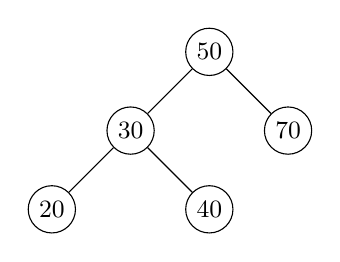
\begin{tikzpicture}[level distance=10mm, sibling distance=20mm,
    every node/.style={circle, draw, minimum size=6mm, inner sep=0pt, font=\small}]
    \node {50}
        child {node {30}
            child {node {20}}
            child {node {40}}
        }
        child {node {70}};
\end{tikzpicture}
\quad vs. \quad
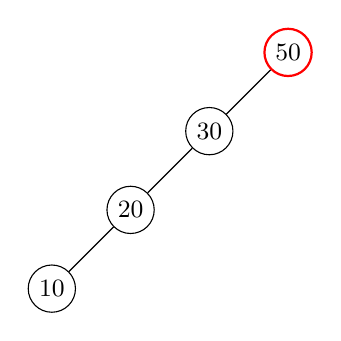
\begin{tikzpicture}[level distance=10mm, sibling distance=20mm,
    every node/.style={circle, draw, minimum size=6mm, inner sep=0pt, font=\small}]
    \node[draw=red, thick] {50}
        child {node {30}
            child {node {20}
                child {node {10}}
                child[missing] {}
            }
            child[missing] {}
        }
        child[missing] {};
\end{tikzpicture}
\end{center}

Left: every node's two subtree heights differ by $\le 1$. \emph{AVL.}

Right: node $50$ has left-subtree height $2$ and right-subtree height $-1$ (null). Balance factor $= 2 - (-1) = 3$. \emph{Not AVL.} Even though $30$ and $20$ would look locally acceptable, the root violates the property.

\subsection*{Height guarantee}

Why does this restriction matter? Because it forces $h = O(\log n)$.

\begin{defnbox}[Fibonacci bound on AVL height]
An AVL tree with $n$ nodes has height $h \le 1.44 \log_2(n+2)$ in the worst case -- about 1.44 times the theoretical minimum. In practice it's even tighter.
\end{defnbox}

The proof uses the minimum-node AVL tree at each height: the smallest AVL of height $h$ has $N(h)$ nodes where $N(h) = N(h-1) + N(h-2) + 1$, the Fibonacci recurrence. Inverting this gives $h \le 1.44 \log_2 n + O(1)$. The 1.44 constant is the price you pay for AVL-balanced instead of perfectly-balanced -- cheap, and well worth it since perfect balance is unreachable during live insertion/removal.

Compare:
\begin{center}
\begin{tabular}{rll}
$n$ & Min height (perfect) & AVL max height \\
\hline
$1\,000$        & 9  & 14 \\
$1\,000\,000$   & 19 & 28 \\
$10^9$          & 29 & 43 \\
\end{tabular}
\end{center}

So even in the worst case, an AVL tree operation on a billion keys costs at most 43 comparisons -- still emphatically $O(\log n)$, not even close to the raw BST's potential $10^9$.

\subsection*{Storing height at each node}

AVL algorithms need to compute balance factors cheaply. Computing a subtree's height by recursively walking it is $O(n)$ -- unaffordable when insert/remove has to check balance factors at every ancestor. The fix: \textbf{cache the height at each node.}

\begin{lstlisting}
template <typename T>
struct AVLNode {
    T          data;
    AVLNode*   left   = nullptr;
    AVLNode*   right  = nullptr;
    AVLNode*   parent = nullptr;   // usually wanted for retrace (section 9.3)
    int        height = 0;         // height of THIS subtree; null children = -1
};

template <typename T>
int height(const AVLNode<T>* n) { return n ? n->height : -1; }

template <typename T>
int balanceFactor(const AVLNode<T>* n) {
    return height(n->left) - height(n->right);
}
\end{lstlisting}

With height stored in the node, balance factor is $O(1)$. The cost: after every structural change (insertion, rotation, removal) we must \emph{recompute the height of every affected ancestor.} This recomputation is why AVL needs parent pointers (or an iterative walk back up from the modified node).

\subsection*{Updating heights after a change}

When node $X$ changes (gains a child, loses one, is rotated), the heights of $X$ and every ancestor up to the root may change. Update rule:
\[
\text{height}(X) = 1 + \max(\text{height}(X.\text{left}), \text{height}(X.\text{right}))
\]
Apply from $X$ upward toward the root. As soon as you reach an ancestor whose height didn't change, you can stop -- the heights further up are unaffected.

\begin{center}
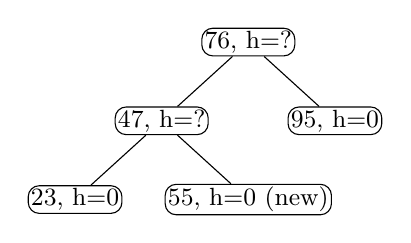
\begin{tikzpicture}[level distance=10mm, sibling distance=22mm,
    every node/.style={rectangle, draw, rounded corners, inner sep=1pt, font=\small}]
    \node {76, h=?}
        child {node {47, h=?}
            child {node {23, h=0}}
            child {node {55, h=0 (new)}}
        }
        child {node {95, h=0}};
\end{tikzpicture}
\end{center}

Insert $55$ under $47$. After the insertion: $55$ is a leaf, $h=0$. At $47$: $\max(0, 0) + 1 = 1$. At $76$: $\max(1, 0) + 1 = 2$. Balance factors: $47$ has $0$, $76$ has $1 - 0 = 1$. Still $\in \{-1, 0, +1\}$ everywhere. Still AVL.

\begin{ideabox}
The stored-height trick is what makes AVL practical. Without it, every insert would need an $O(n)$ rescan of subtree heights to verify balance. With it, the per-insert rebalancing cost stays $O(\log n)$ because you only touch ancestors on one root-to-leaf path.
\end{ideabox}

\subsection*{Why this invariant, and not something else?}

The ``differ by at most 1'' constraint is a specific compromise:
\begin{itemize}[leftmargin=*]
    \item \textbf{Stricter} (``differ by at most 0'' = perfectly balanced): impossible to maintain under arbitrary insertion, because you can't turn $N = 3$ into $N = 4$ with perfect symmetry.
    \item \textbf{Looser} (``differ by at most 2'' or more): allows more imbalance before triggering rebalancing, but height grows faster and search slows down.
    \item \textbf{$\pm 1$}: tightest strictness that can be maintained with a constant number of local rotations after each modification. It's the sweet spot.
\end{itemize}

Red-black trees (the main chapter splits roughly evenly: \S9.1--\S9.4 AVL, \S9.5--\S9.8 red-black) use a weaker balance invariant that allows larger height differences but cheaper rebalancing. They're strictly less balanced than AVL (worst-case height $\sim 2 \log n$ vs.\ AVL's $1.44 \log n$), but their rebalancing has lower overhead on average. \texttt{std::map} uses red-black; competitive programmers and strict-performance workloads sometimes prefer AVL.

\subsection*{Road map for chapter 9}

Sections 9.2--9.7 formalize rotations (the single primitive AVL uses to fix violations), give the full insert/remove algorithms, and walk through the four rebalancing cases (left-left, left-right, right-right, right-left). This section established \emph{what} AVL is; the rest of the chapter is \emph{how}.

\begin{warnbox}
Don't conflate AVL's balance factor with red-black's node colors. Both are auxiliary per-node state used to maintain structural invariants, but they encode different constraints and trigger different rebalancing rules. AVL says ``left minus right height is in $\{-1, 0, +1\}$.'' Red-black says ``no red node has a red child, and every path from root to any null has the same number of black nodes.'' Different invariants, different rotations, different use cases.
\end{warnbox}

\section{9.2 Rotations: The Only Primitive AVL Needs}

Section 9.1 said ``we restore balance with local rotations.'' This section defines the rotation precisely and gives all the helper procedures AVL operations will need. One operation -- the \textbf{rotation} -- is the whole mechanical toolkit. AVL insert, AVL remove, and AVL rebalance all boil down to ``figure out which rotation to apply, then apply it.''

\begin{defnbox}[Rotation]
A rotation is a local rearrangement of a BST that \emph{changes the shape} of a subtree while \emph{preserving the in-order (BST) ordering} of its keys. Every other tree invariant (heights, parent pointers) must be updated by the rotation code. BST ordering is the one property that survives automatically.
\end{defnbox}

Rotations were teased in chapter 7.5 with treaps -- same operation, different trigger. In a treap the trigger is ``a child has a higher priority than its parent.'' In an AVL tree the trigger is ``this node's balance factor is $\pm 2$.'' The rotation primitive is identical in both.

\subsection*{Right rotation}

A \textbf{right rotation at node $D$} requires $D$ to have a left child $B$. After the rotation, $B$ is the new subtree root and $D$ becomes $B$'s right child. $B$'s former right child (call it $C$) becomes $D$'s new left child -- that's the move that preserves BST ordering.

\begin{center}
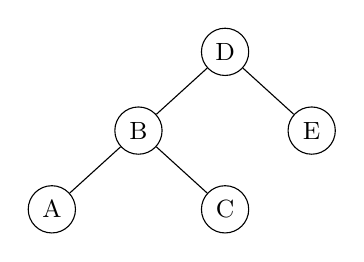
\begin{tikzpicture}[level distance=10mm, sibling distance=22mm,
    every node/.style={circle, draw, minimum size=6mm, inner sep=0pt, font=\small}]
    \node {D}
        child {node {B}
            child {node {A}}
            child {node {C}}
        }
        child {node {E}};
\end{tikzpicture}
\quad $\xrightarrow{\text{rotate right at } D}$ \quad
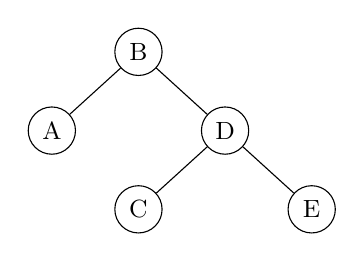
\begin{tikzpicture}[level distance=10mm, sibling distance=22mm,
    every node/.style={circle, draw, minimum size=6mm, inner sep=0pt, font=\small}]
    \node {B}
        child {node {A}}
        child {node {D}
            child {node {C}}
            child {node {E}}
        };
\end{tikzpicture}
\end{center}

Ordering check: before the rotation, the in-order sequence is $A, B, C, D, E$. After: $A, B, C, D, E$. Identical -- rotations are \emph{identity on in-order sequence}. Height behavior: if the original tree was left-heavy (left subtree taller), the rotation reduces the height difference; that's why this fixes AVL violations on the left side.

The generalization to subtrees (not just single nodes) is what makes rotations useful for arbitrary tree sizes:

\begin{center}
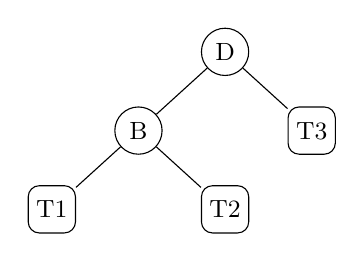
\begin{tikzpicture}[level distance=10mm, sibling distance=22mm,
    every node/.style={circle, draw, minimum size=6mm, inner sep=0pt, font=\small}]
    \node {D}
        child {node {B}
            child {node[rectangle, rounded corners] {T1}}
            child {node[rectangle, rounded corners] {T2}}
        }
        child {node[rectangle, rounded corners] {T3}};
\end{tikzpicture}
\quad $\to$ \quad
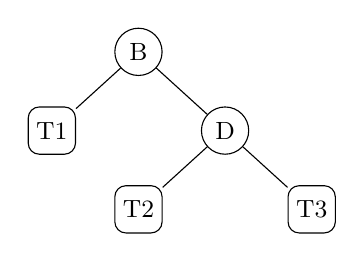
\begin{tikzpicture}[level distance=10mm, sibling distance=22mm,
    every node/.style={circle, draw, minimum size=6mm, inner sep=0pt, font=\small}]
    \node {B}
        child {node[rectangle, rounded corners] {T1}}
        child {node {D}
            child {node[rectangle, rounded corners] {T2}}
            child {node[rectangle, rounded corners] {T3}}
        };
\end{tikzpicture}
\end{center}

$T_1, T_2, T_3$ are arbitrary subtrees. The rotation only rewires three pointers at the top; the subtrees ride along unchanged. That's why each rotation is $O(1)$.

\subsection*{Left rotation}

The mirror image: a \textbf{left rotation at node $D$} requires $D$ to have a right child. It promotes the right child to the subtree root.

\begin{center}
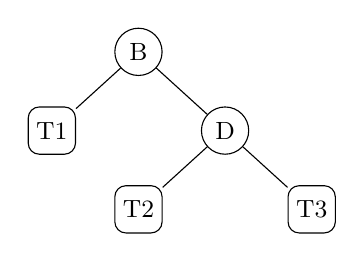
\begin{tikzpicture}[level distance=10mm, sibling distance=22mm,
    every node/.style={circle, draw, minimum size=6mm, inner sep=0pt, font=\small}]
    \node {B}
        child {node[rectangle, rounded corners] {T1}}
        child {node {D}
            child {node[rectangle, rounded corners] {T2}}
            child {node[rectangle, rounded corners] {T3}}
        };
\end{tikzpicture}
\quad $\xrightarrow{\text{rotate left at } B}$ \quad
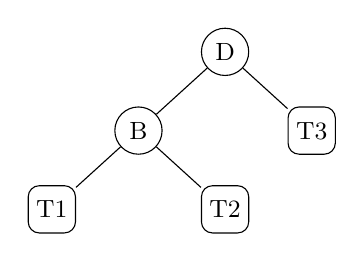
\begin{tikzpicture}[level distance=10mm, sibling distance=22mm,
    every node/.style={circle, draw, minimum size=6mm, inner sep=0pt, font=\small}]
    \node {D}
        child {node {B}
            child {node[rectangle, rounded corners] {T1}}
            child {node[rectangle, rounded corners] {T2}}
        }
        child {node[rectangle, rounded corners] {T3}};
\end{tikzpicture}
\end{center}

A left rotation is literally the inverse of the matching right rotation.

\subsection*{Utility: update-height, set-child, replace-child, balance-factor}

Before showing rotation code, we need the housekeeping helpers. These all operate on \texttt{AVLNode<T>} from section 9.1 (with cached \texttt{height} and \texttt{parent} fields).

\begin{lstlisting}
template <typename T>
void avlUpdateHeight(AVLNode<T>* n) {
    int lh = (n->left  != nullptr) ? n->left->height  : -1;
    int rh = (n->right != nullptr) ? n->right->height : -1;
    n->height = 1 + std::max(lh, rh);
}

template <typename T>
int avlBalance(const AVLNode<T>* n) {
    int lh = (n->left  != nullptr) ? n->left->height  : -1;
    int rh = (n->right != nullptr) ? n->right->height : -1;
    return lh - rh;
}

// Set `child` as parent's left/right. Fix child's parent pointer.
// Recompute parent's cached height.
template <typename T>
void avlSetChild(AVLNode<T>* parent, bool isLeft, AVLNode<T>* child) {
    if (isLeft) parent->left = child;
    else        parent->right = child;
    if (child != nullptr) child->parent = parent;
    avlUpdateHeight(parent);
}

template <typename T>
void avlReplaceChild(AVLNode<T>* parent,
                     AVLNode<T>* currentChild,
                     AVLNode<T>* newChild) {
    if (parent->left == currentChild)  avlSetChild(parent, true,  newChild);
    else                               avlSetChild(parent, false, newChild);
}
\end{lstlisting}

\texttt{avlSetChild} does the \emph{four} things you always forget together: (1) wire parent's child slot, (2) wire child's parent pointer, (3) the caller picks which slot, (4) recompute height. Any AVL implementation that tries to inline these will eventually get them out of sync and ship a bug.

\subsection*{Right rotation algorithm}

\begin{lstlisting}
template <typename T>
AVLNode<T>* avlRotateRight(AVLNode<T>*& root, AVLNode<T>* D) {
    AVLNode<T>* B  = D->left;          // must be non-null
    AVLNode<T>* BR = B->right;         // "C" in the diagram -- may be null

    if (D->parent != nullptr) avlReplaceChild(D->parent, D, B);
    else                      { root = B; B->parent = nullptr; }

    avlSetChild(B, false, D);          // B's new right is D
    avlSetChild(D, true,  BR);         // D's new left is B's old right
    return B;                          // B is the new subtree root
}
\end{lstlisting}

Three rewires at the top of the subtree, heights recomputed as part of each \texttt{setChild}, and we return the new root so callers can continue walking upward if needed.

\subsection*{Left rotation algorithm}

Symmetric -- swap every ``left'' for ``right'':

\begin{lstlisting}
template <typename T>
AVLNode<T>* avlRotateLeft(AVLNode<T>*& root, AVLNode<T>* B) {
    AVLNode<T>* D  = B->right;
    AVLNode<T>* DL = D->left;

    if (B->parent != nullptr) avlReplaceChild(B->parent, B, D);
    else                      { root = D; D->parent = nullptr; }

    avlSetChild(D, true,  B);
    avlSetChild(B, false, DL);
    return D;
}
\end{lstlisting}

\subsection*{The rebalance procedure}

After any insertion or removal, walk from the modified node up to the root; at each ancestor, update its cached height and check its balance factor. If the balance factor is $\pm 2$, apply one or two rotations to fix it. This is the procedure. All four cases (left-left, left-right, right-right, right-left) flow through it:

\begin{lstlisting}
template <typename T>
AVLNode<T>* avlRebalance(AVLNode<T>*& root, AVLNode<T>* n) {
    avlUpdateHeight(n);
    int bf = avlBalance(n);

    if (bf == 2) {                              // left-heavy
        if (avlBalance(n->left) == -1)          // left-right case: pre-rotate
            avlRotateLeft(root, n->left);
        return avlRotateRight(root, n);
    }
    if (bf == -2) {                             // right-heavy
        if (avlBalance(n->right) == 1)          // right-left case: pre-rotate
            avlRotateRight(root, n->right);
        return avlRotateLeft(root, n);
    }
    return n;                                   // -1, 0, or 1: already balanced
}
\end{lstlisting}

The two inner checks detect the \emph{double-rotation cases}. If the left child's balance factor has the opposite sign from the parent's (i.e., $\text{bf}(n.\text{left}) = -1$ when $\text{bf}(n) = +2$), a single right rotation at $n$ would not fix the imbalance -- we first left-rotate $n$'s left child to turn a ``zig-zag'' into a ``zig-zig'', then right-rotate $n$. These are the four cases, collapsed into six lines of code.

\subsection*{The four imbalance cases}

\begin{center}
\begin{tabular}{lll}
Name  & Trigger (balance factors)    & Fix \\
\hline
Left-Left   & $\text{bf}(n) = +2$, $\text{bf}(n.\text{left}) \ge 0$   & single right-rotate at $n$ \\
Left-Right  & $\text{bf}(n) = +2$, $\text{bf}(n.\text{left}) = -1$    & left-rotate at $n.\text{left}$, then right-rotate at $n$ \\
Right-Right & $\text{bf}(n) = -2$, $\text{bf}(n.\text{right}) \le 0$  & single left-rotate at $n$ \\
Right-Left  & $\text{bf}(n) = -2$, $\text{bf}(n.\text{right}) = +1$   & right-rotate at $n.\text{right}$, then left-rotate at $n$ \\
\end{tabular}
\end{center}

Left-Left and Right-Right are the ``easy'' cases: the imbalance is already aligned and a single rotation fixes it. Left-Right and Right-Left are the ``zig-zag'' cases: the imbalance is shaped like a kink in the path from parent to grandchild, and you first rotate to straighten the kink, then rotate again to fix the height.

\begin{ideabox}
Notice the elegance: two rotation primitives (left, right), four named cases (LL, LR, RR, RL), but the rebalance procedure decides which to apply with a single check on the balance factor of the child along the heavy side. You don't name cases in code -- the balance factors pick the right rotation(s) automatically.
\end{ideabox}

\begin{warnbox}
Every rotation and setChild updates cached heights \emph{locally}. The caller is responsible for continuing the retrace -- walking up to the next ancestor and calling \texttt{avlRebalance} there too, because a rotation at a child can still leave an ancestor further up imbalanced. Section 9.3 (or wherever the insert algorithm lives) shows that loop.
\end{warnbox}

\begin{notebox}
\textbf{Rotations are universal.} A theoretical claim worth knowing
even though we never use it algorithmically: \emph{$O(n)$ rotations
suffice to transform any binary tree into any other binary tree on
the same multiset of keys, as long as both have the same in-order
sequence.} Proof sketch: repeatedly apply the last possible right
rotation (root has a left child, descend into the right spine, then
right-rotate at the deepest node with a left child) until you
reach a canonical right-spine ``chain'' of $n$ nodes. That takes at
most $n - 1$ rotations. From the chain you can reach any target
shape by reversing the same procedure on the target. So
$2(n-1) = O(n)$ rotations are always enough. The takeaway is not
the bound itself (we'll do much better -- AVL needs only $O(\log n)$
rotations per operation) but the \emph{adequacy} answer: rotations
\emph{are} a powerful enough primitive to maintain any
shape-based invariant on a BST without leaving the rotations-only
regime. Chapter 11's B-trees use the analogous primitive
(split / merge of sibling nodes), which is universal in the same
sense for $B$-ary trees.
\end{notebox}

\subsection*{Why rotations alone are sufficient}

It's worth marveling at: every AVL rebalancing is one or two rotations. The shape adjustment you need to fix an imbalance is always local -- contained within a grandparent-parent-child trio -- because AVL has such a tight invariant that violations can't be more than height-two deep before they're caught. This is what makes AVL fast: worst-case two rotations per insert, one rotation per removal iteration. All $O(1)$ per fix; walking back up the tree is $O(\log n)$, giving $O(\log n)$ total per modification.

\section{9.3 AVL Insertion}

Section 9.2 gave us the rotation primitives; this section assembles them into a full insertion algorithm. The structure is simple to state and slightly fiddly to implement:

\begin{defnbox}[AVL insertion]
\begin{enumerate}[leftmargin=*]
    \item \textbf{Insert} the new node using the standard BST insertion (walk down, attach at the first empty child slot).
    \item \textbf{Retrace} upward from the new node's parent. At each ancestor, update the cached height and check the balance factor.
    \item \textbf{Rebalance} on the first node whose balance factor is $\pm 2$. Apply one or two rotations; this restores the invariant for the entire path below. Continue retracing because a rotation can change the subtree height, which can expose further imbalance higher up.
\end{enumerate}
\end{defnbox}

\subsection*{Retrace: what changes when}

Inserting a leaf $L$ increases the height of some ancestors by 1 but not others. Specifically, the height of $L$'s parent $P$ becomes $h_P' = \max(h_P, 0) + 1$. If $P$ previously had a non-null sibling child at the same height, $P$'s height doesn't change -- the new node just filled the other slot. If $P$ was a leaf before, $P$'s height increased from $0$ to $1$, and that change propagates upward.

This cascading-height behavior is why we walk all the way up: we don't know in advance how far the height increase propagates. We stop propagating (for height-update purposes) at the first ancestor whose height didn't change. But for balance-factor checking we still walk all the way up -- even if heights stabilize, a descendant rotation can shift things.

The canonical recipe is simpler in code: ``walk to root, call \texttt{avlRebalance} at every ancestor.'' \texttt{avlRebalance} updates height and checks balance factor on its own, so a single procedure does both jobs.

\subsection*{The four insertion cases (by imbalance shape)}

After inserting, the first unbalanced ancestor $P$ (balance factor $\pm 2$) is fixed by one of four cases, named for the direction to the grandchild where the insertion happened:

\begin{center}
\begin{tabular}{lll}
Shape       & Signal                       & Fix \\
\hline
Left-Left   & bf$(P) = +2$, bf$(P.\text{left}) \ge 0$  & right-rotate at $P$ \\
Left-Right  & bf$(P) = +2$, bf$(P.\text{left}) = -1$   & left-rotate at $P.\text{left}$, then right-rotate at $P$ \\
Right-Right & bf$(P) = -2$, bf$(P.\text{right}) \le 0$ & left-rotate at $P$ \\
Right-Left  & bf$(P) = -2$, bf$(P.\text{right}) = +1$  & right-rotate at $P.\text{right}$, then left-rotate at $P$ \\
\end{tabular}
\end{center}

Left-Left and Right-Right are ``straight'' imbalances: the insertion went deeper on an already-heavy side, and a single rotation fixes the heights. Left-Right and Right-Left are ``zig-zag'' imbalances where the first rotation \emph{straightens} the shape into a Left-Left or Right-Right, and the second rotation then fixes it.

\subsection*{Left-Left example}

Insert 12 into this tree:

\begin{center}
\emph{Before:}
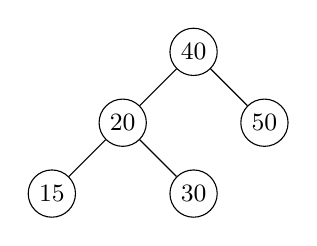
\begin{tikzpicture}[level distance=9mm, sibling distance=18mm,
    every node/.style={circle, draw, minimum size=6mm, inner sep=0pt, font=\small}]
    \node {40}
        child {node {20}
            child {node {15}
                child[missing] {}
                child[missing] {}
            }
            child {node {30}}
        }
        child {node {50}};
\end{tikzpicture}
\quad $\to$ \emph{after insert 12, before rebalance:}
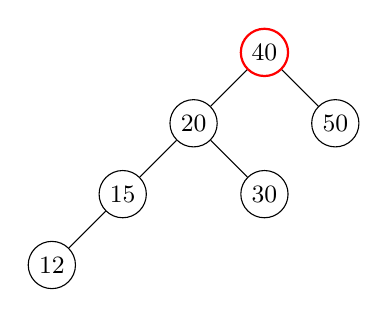
\begin{tikzpicture}[level distance=9mm, sibling distance=18mm,
    every node/.style={circle, draw, minimum size=6mm, inner sep=0pt, font=\small}]
    \node[draw=red, thick] {40}
        child {node {20}
            child {node {15}
                child {node {12}}
                child[missing] {}
            }
            child {node {30}}
        }
        child {node {50}};
\end{tikzpicture}
\end{center}

After insertion, height of $20$ is $2$, height of $50$ is $0$. bf$(40) = 2 - 0 = 2$. Problem. $P = 40$, $P.\text{left} = 20$, bf$(20) = 1 - 0 = 1 \ge 0$: \textbf{Left-Left case}. Single right-rotate at $40$:

\begin{center}
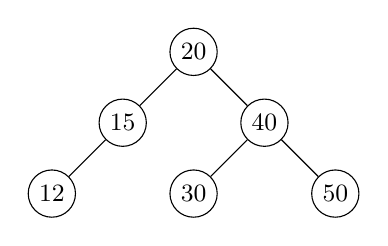
\begin{tikzpicture}[level distance=9mm, sibling distance=18mm,
    every node/.style={circle, draw, minimum size=6mm, inner sep=0pt, font=\small}]
    \node {20}
        child {node {15}
            child {node {12}}
            child[missing] {}
        }
        child {node {40}
            child {node {30}}
            child {node {50}}
        };
\end{tikzpicture}
\end{center}

Every balance factor is now in $\{-1, 0, +1\}$. Tree is back to AVL in one rotation.

\subsection*{Left-Right example (the double-rotation case)}

Insert 38 into this tree:

\begin{center}
\emph{Before:}
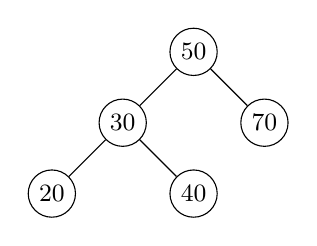
\begin{tikzpicture}[level distance=9mm, sibling distance=18mm,
    every node/.style={circle, draw, minimum size=6mm, inner sep=0pt, font=\small}]
    \node {50}
        child {node {30}
            child {node {20}}
            child {node {40}}
        }
        child {node {70}};
\end{tikzpicture}
\quad $\to$ \emph{after insert 38:}
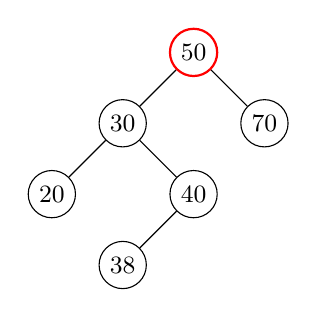
\begin{tikzpicture}[level distance=9mm, sibling distance=18mm,
    every node/.style={circle, draw, minimum size=6mm, inner sep=0pt, font=\small}]
    \node[draw=red, thick] {50}
        child {node {30}
            child {node {20}}
            child {node {40}
                child {node {38}}
                child[missing] {}
            }
        }
        child {node {70}};
\end{tikzpicture}
\end{center}

bf$(50) = 2$, bf$(30) = -1$: \textbf{Left-Right case}. Two-step fix:
\begin{enumerate}[leftmargin=*]
    \item Left-rotate at $30$ (the left child). This straightens the L-R zig-zag.
    \item Right-rotate at $50$.
\end{enumerate}

After step 1 (left-rotate at $30$):

\begin{center}
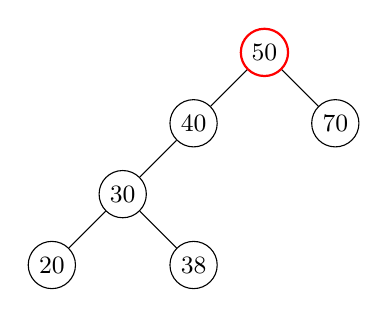
\begin{tikzpicture}[level distance=9mm, sibling distance=18mm,
    every node/.style={circle, draw, minimum size=6mm, inner sep=0pt, font=\small}]
    \node[draw=red, thick] {50}
        child {node {40}
            child {node {30}
                child {node {20}}
                child {node {38}}
            }
            child[missing] {}
        }
        child {node {70}};
\end{tikzpicture}
\end{center}

Now the shape is Left-Left (bf$(50) = 2$, bf$(40) = 1$). Step 2, right-rotate at $50$:

\begin{center}
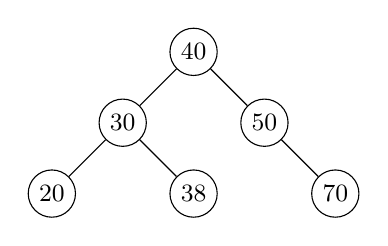
\begin{tikzpicture}[level distance=9mm, sibling distance=18mm,
    every node/.style={circle, draw, minimum size=6mm, inner sep=0pt, font=\small}]
    \node {40}
        child {node {30}
            child {node {20}}
            child {node {38}}
        }
        child {node {50}
            child[missing] {}
            child {node {70}}
        };
\end{tikzpicture}
\end{center}

Balanced. Right-Right and Right-Left are the mirror images.

\subsection*{The insertion algorithm, with retrace}

\begin{lstlisting}
template <typename T>
void avlInsert(AVLNode<T>*& root, AVLNode<T>* node) {
    node->left = node->right = node->parent = nullptr;
    node->height = 0;

    if (root == nullptr) { root = node; return; }

    // Phase 1: standard BST insertion.
    AVLNode<T>* cur = root;
    while (true) {
        if (node->data < cur->data) {
            if (cur->left == nullptr) {
                cur->left = node; node->parent = cur; break;
            }
            cur = cur->left;
        } else {
            if (cur->right == nullptr) {
                cur->right = node; node->parent = cur; break;
            }
            cur = cur->right;
        }
    }

    // Phase 2: retrace. Walk from the parent up to the root,
    // rebalancing each ancestor.
    for (AVLNode<T>* n = node->parent; n != nullptr; n = n->parent) {
        avlRebalance(root, n);
        // After a rotation, n->parent might have changed. Re-read via the
        // node that came out of rebalance; but if rebalance returned the
        // new root, we want to keep going via its parent pointer. The
        // for-loop update reads n->parent, so this works as-is because
        // setChild/rotations keep parent pointers consistent.
    }
}
\end{lstlisting}

Two passes down-then-up, both $O(\log n)$. Inserting a duplicate is handled by the ``$>=$'' branch going right -- equal keys end up in the right subtree.

\subsection*{Cost}

\begin{center}
\begin{tabular}{ll}
Phase          & Cost \\
\hline
BST descent    & $O(\log n)$ (height is AVL-bounded) \\
Retrace        & $O(\log n)$ ancestors visited \\
Rebalance each & $O(1)$ per ancestor (at most 2 rotations total) \\
\hline
\textbf{Total} & $\mathbf{O(\log n)}$ \\
\end{tabular}
\end{center}

Space is $O(1)$ auxiliary (a handful of temporaries for the rotation helpers). Compare this to the raw BST insert in section 6.5: identical descent cost, identical insertion cost, plus an $O(\log n)$ retrace that guarantees the tree never degrades. A small constant-factor tax for a permanent worst-case guarantee.

\subsection*{Why the ``first unbalanced ancestor'' is enough}

An important theorem (not proved in the textbook but worth knowing): \emph{during AVL insertion, fixing the first unbalanced ancestor restores the AVL property everywhere.} Higher ancestors \emph{will} have their cached heights touched during the retrace, but their balance factors will fall back into $\{-1, 0, +1\}$ automatically because a rotation at the first bad ancestor reduces that subtree's height by 1, undoing the height increase the insertion caused.

This is why insertion needs \emph{at most two rotations} total (one pair for the Left-Right or Right-Left case, one for Left-Left or Right-Right). Insertion is cheaper than removal in AVL, which in the worst case may require $O(\log n)$ rotations along the path.

\begin{ideabox}
AVL insert is ``BST insert, then walk back up fixing things.'' That pattern -- descend with intent, ascend to repair -- shows up again in red-black insert, in B-tree split-on-insert, and in persistent data structures. Every self-balancing structure makes the descent cheap, stores some auxiliary state at each node, and pays the $O(\log n)$ ascent to reconcile after modification.
\end{ideabox}

\subsection*{Phone book: why AVL matters}

The motivating example is a phone book loaded from already-sorted names. In a raw BST this is the pathological case -- height grows to $N - 1$. In an AVL tree, each insertion may trigger a rotation, and after loading $N$ sorted keys you end up with height $\approx \log_2 N$, even though no permutation-shuffling happened. The AVL invariant silently transforms a degenerate input into a balanced structure, at a cost of one or two rotations per insert.

\begin{warnbox}
Be careful about equal-key handling. The code above sends equal keys to the right subtree. This is consistent but not \emph{stable} (insertion order among equal keys isn't preserved). For applications that need stable ordering, store a tiebreaker (like insertion sequence number) in the comparison key, or use a \texttt{multiset}-style structure that tracks insertion order separately.
\end{warnbox}

\begin{examplebox}
\textbf{Worked AVL insertion sequence: $10, 20, 30, 40, 50, 25$.}
Trace each insert into an initially empty AVL tree, showing the
balance factor at every node after the insert and identifying which
case (if any) fires. We use the convention bf$(\cdot)$ from \S9.1.

\textbf{Frame 1 -- insert $10$.} Empty tree. $10$ becomes the root.
\[
10 \quad (\text{bf} = 0)
\]
No imbalance.

\textbf{Frame 2 -- insert $20$.} $20 > 10$, attach as right child.
\[
10 \,(\text{bf} = -1) \to \text{right} \to 20 \,(\text{bf} = 0)
\]
bf$(10) = -1$, still in $\{-1, 0, +1\}$. No rotation.

\textbf{Frame 3 -- insert $30$.} $30 > 10$, then $30 > 20$, attach
as right child of $20$.
\[
10 \,(\text{bf} = -2) \to 20 \,(\text{bf} = -1) \to 30 \,(\text{bf} = 0)
\]
First unbalanced ancestor on retrace is $10$ (bf $= -2$).
bf$(10.\text{right}) = $ bf$(20) = -1 \le 0$ $\Rightarrow$
\textbf{Right-Right case}. Single \emph{left}-rotate at $10$:
\[
20 \,(\text{bf} = 0) \,\,\,\text{with}\,\,\, \text{left} = 10 \,(\text{bf} = 0),\, \text{right} = 30 \,(\text{bf} = 0).
\]

\textbf{Frame 4 -- insert $40$.} BST descent: $40 > 20$, $40 > 30$,
attach as right child of $30$. After insert:
\[
20 \,(\text{bf} = -1),\,\, 10 \,(\text{bf} = 0),\,\, 30 \,(\text{bf} = -1),\,\, 40 \,(\text{bf} = 0).
\]
All balance factors in $\{-1, 0, +1\}$. No rotation.

\textbf{Frame 5 -- insert $50$.} BST descent: $50 > 20$, $50 > 30$,
$50 > 40$, attach as right child of $40$. After insert:
\[
20 \,(\text{bf} = -2),\,\, 30 \,(\text{bf} = -2),\,\, 40 \,(\text{bf} = -1),\,\, 50 \,(\text{bf} = 0).
\]
Retrace from $40$ upward. First imbalance hit is $30$ (bf $= -2$).
bf$(30.\text{right}) = $ bf$(40) = -1 \le 0$ $\Rightarrow$
\textbf{Right-Right case}. Left-rotate at $30$:
\[
\begin{array}{l}
20 \,(\text{bf} = ?) \\
\quad \text{left}: 10 \\
\quad \text{right}: 40 \,(\text{bf} = 0) \\
\qquad \text{left}: 30 \,(\text{bf} = 0), \text{right}: 50 \,(\text{bf} = 0)
\end{array}
\]
After the rotation, $20$'s right subtree shrank by 1 in height, so
bf$(20)$ recomputes to $-1$. Done.

\textbf{Frame 6 -- insert $25$.} BST descent: $25 > 20$, $25 < 40$,
$25 < 30$, attach as left child of $30$. After insert:
\[
\begin{array}{l}
20 \,(\text{bf} = -2) \\
\quad \text{left}: 10 \,(\text{bf} = 0) \\
\quad \text{right}: 40 \,(\text{bf} = +1) \\
\qquad \text{left}: 30 \,(\text{bf} = +1) \\
\qquad\quad \text{left}: 25 \,(\text{bf} = 0) \\
\qquad \text{right}: 50 \,(\text{bf} = 0)
\end{array}
\]
Retrace from $25$ upward. $30$ is balanced (bf $= +1$); $40$ is
balanced (bf $= +1$); $20$ is unbalanced (bf $= -2$). Now the
discriminator: bf$(20.\text{right}) = $ bf$(40) = +1$. Right child
balance factor has \emph{opposite sign} from parent's
$\Rightarrow$ \textbf{Right-Left case} (the LR mirror). Two-rotation
fix: right-rotate at $40$, then left-rotate at $20$.

After right-rotate at $40$:
\[
\begin{array}{l}
20 \,(\text{bf} = -2) \\
\quad \text{left}: 10 \\
\quad \text{right}: 30 \,(\text{bf} = -1) \\
\qquad \text{left}: 25, \text{right}: 40 \,(\text{bf} = -1) \\
\qquad\qquad \text{right}: 50
\end{array}
\]
Now the shape is Right-Right (bf$(20) = -2$, bf$(30) = -1$).
Left-rotate at $20$:
\[
\begin{array}{l}
30 \,(\text{bf} = 0) \\
\quad \text{left}: 20 \,(\text{bf} = 0) \\
\qquad \text{left}: 10, \text{right}: 25 \\
\quad \text{right}: 40 \,(\text{bf} = -1) \\
\qquad \text{right}: 50
\end{array}
\]
All balance factors in $\{-1, 0, +1\}$. Tree is balanced.

\textbf{Takeaway.} Six inserts; three rotations total ($1$ single
on insert $30$, $1$ single on insert $50$, $1$ double on insert
$25$). The double-rotation case at insert $25$ is the
\textbf{LL/LR boundary}: had the insert been $35$ instead (right of
$30$ rather than left), case $30$'s child balance factor would have
been $-1$ and the same RR-case left-rotate as on insert $50$ would
have sufficed. The LR/RL cases are precisely the
``imbalance kink'' cases where the insertion went to the
\emph{inner} grandchild rather than the outer.
\end{examplebox}

\section{9.4 AVL Removal}

Removal is where AVL earns a slightly worse worst-case-rotation count than insertion. For insertion, at most one cascade (one single or one double rotation) handles everything. For removal, a single rotation can \emph{shorten} a subtree, which can trigger another imbalance one level up, which can trigger another, and so on -- up to $O(\log n)$ rotations along the retrace path.

\begin{defnbox}[AVL removal]
\begin{enumerate}[leftmargin=*]
    \item \textbf{BST-remove} the node using the standard four-case algorithm from chapter 6: leaf, single-child, two-children (copy-successor-then-remove), root-specialization.
    \item \textbf{Retrace} upward from the parent of the physically-removed node. At each ancestor, call \texttt{avlRebalance} to update the cached height and apply 0, 1, or 2 rotations as needed.
    \item Continue retracing to the root. Unlike insertion, you \emph{cannot} stop at the first fix -- removal-induced height decreases can propagate arbitrarily far.
\end{enumerate}
\end{defnbox}

\subsection*{The two-children shortcut}

Chapter~6 \S6.6 showed that removing a node with two children is handled by copying the in-order successor's data over the doomed node, then recursively removing the successor. That trick still works for AVL -- the successor always has at most one child (it's the leftmost of the right subtree), so the recursive call lands in the leaf / one-child case and rebalances from there. Recursion handles the retrace; you don't need to rebalance twice.

\subsection*{The algorithm}

\begin{lstlisting}
template <typename T>
bool avlRemoveNode(AVLNode<T>*& root, AVLNode<T>* node) {
    if (node == nullptr) return false;

    // Case 1: two children -- copy successor's data, recurse to remove it.
    if (node->left != nullptr && node->right != nullptr) {
        AVLNode<T>* succ = node->right;
        while (succ->left != nullptr) succ = succ->left;
        node->data = succ->data;
        return avlRemoveNode(root, succ);
    }

    AVLNode<T>* parent = node->parent;
    AVLNode<T>* only   = (node->left != nullptr) ? node->left : node->right;

    // Case 2: node is the root (0 or 1 child).
    if (node == root) {
        root = only;
        if (root != nullptr) root->parent = nullptr;
    }
    // Cases 3 & 4: splice `only` (possibly null) into node's slot below parent.
    else {
        avlReplaceChild(parent, node, only);
    }

    delete node;

    // Retrace: walk up from parent to root, rebalancing every ancestor.
    for (AVLNode<T>* n = parent; n != nullptr; n = n->parent) {
        avlRebalance(root, n);
    }
    return true;
}

template <typename T>
bool avlRemoveKey(AVLNode<T>*& root, const T& key) {
    AVLNode<T>* node = bstSearch(root, key);
    return avlRemoveNode(root, node);
}
\end{lstlisting}

Notice the retrace walks \emph{all the way} to the root. For insertion, we could stop at the first rebalanced ancestor; for removal, we can't. A single rotation might fix one level and shorten the subtree, which exposes a new imbalance at the next level up.

\subsection*{Why removal can cascade}

\begin{center}
Consider a narrow AVL tree where a rebalancing rotation reduces a subtree's height by 1. That subtree's parent, which was balanced before, might now see bf $= \pm 2$ and need its own rotation. That rotation might again reduce height by 1 and propagate.
\end{center}

In the worst case this cascade runs the entire height of the tree, so $O(\log n)$ rotations. Each rotation is $O(1)$, so total cost is $O(\log n)$. Still logarithmic; just a slightly worse constant than insertion.

\subsection*{Walk-through: simple rotation after removal}

Start with this AVL tree and remove node $93$:

\begin{center}
\emph{Before:}
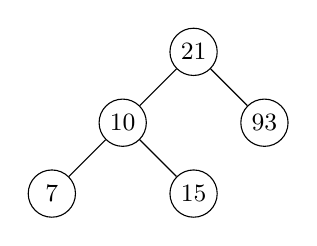
\begin{tikzpicture}[level distance=9mm, sibling distance=18mm,
    every node/.style={circle, draw, minimum size=6mm, inner sep=0pt, font=\small}]
    \node {21}
        child {node {10}
            child {node {7}}
            child {node {15}}
        }
        child {node {93}};
\end{tikzpicture}
\end{center}

After removing $93$ (case 1 -- leaf), the right subtree of $21$ is null. Height of $21$'s left subtree is $1$, right is $-1$. bf$(21) = 1 - (-1) = 2$. \textbf{Left-Left imbalance} (bf$(10) = 0$ -- note this counts as Left-Left because the condition on the child is bf $\ge 0$). Right-rotate at $21$:

\begin{center}
\emph{After:}
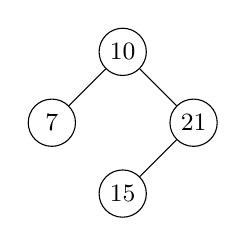
\begin{tikzpicture}[level distance=9mm, sibling distance=18mm,
    every node/.style={circle, draw, minimum size=6mm, inner sep=0pt, font=\small}]
    \node {10}
        child {node {7}}
        child {node {21}
            child {node {15}}
            child[missing] {}
        };
\end{tikzpicture}
\end{center}

All balance factors in $\{-1, 0, +1\}$. Done.

\subsection*{Walk-through: successor case}

Remove $84$ from:

\begin{center}
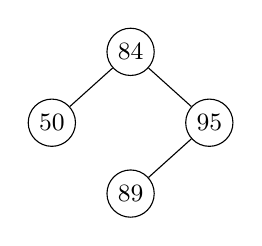
\begin{tikzpicture}[level distance=9mm, sibling distance=20mm,
    every node/.style={circle, draw, minimum size=6mm, inner sep=0pt, font=\small}]
    \node {84}
        child {node {50}
            child[missing] {}
            child[missing] {}
        }
        child {node {95}
            child {node {89}}
            child[missing] {}
        };
\end{tikzpicture}
\end{center}

Node $84$ has two children. Successor = leftmost of right subtree = $89$. Copy $89$'s data over $84$, then recursively remove $89$ (which is now a leaf at its original position):

\begin{center}
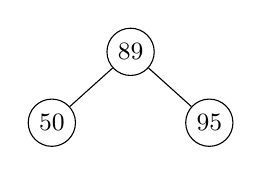
\begin{tikzpicture}[level distance=9mm, sibling distance=20mm,
    every node/.style={circle, draw, minimum size=6mm, inner sep=0pt, font=\small}]
    \node {89}
        child {node {50}}
        child {node {95}
            child[missing] {}
            child[missing] {}
        };
\end{tikzpicture}
\end{center}

Retrace from $95$ (where $89$ was attached): bf$(95) = -1 - (-1) = 0$. bf$(89$, the new root$) = 0 - 0 = 0$. No rotations. Tree is balanced. Notice: the successor copy only moves data, not the node itself; all parent/child relationships stay intact below.

\subsection*{Cost}

\begin{center}
\begin{tabular}{ll}
Phase              & Cost \\
\hline
BST search + remove & $O(\log n)$ \\
Retrace             & $O(\log n)$ ancestors \\
Rotations along retrace & Up to $O(\log n)$ total (each $O(1)$) \\
\hline
\textbf{Total}      & $\mathbf{O(\log n)}$ \\
\end{tabular}
\end{center}

Still $O(\log n)$. The worst-case \emph{rotation count} is higher than insertion's (up to $O(\log n)$ instead of at most 2), but each rotation is still constant work and the retrace path is the same length.

\begin{ideabox}
Insertion gets a rebalancing ``freebie'' because a single rotation restores the original pre-insertion height -- propagation stops. Removal doesn't: a rotation reduces the subtree's height by one, which is the whole problem being cascaded upward. This asymmetry is fundamental to self-balancing trees; red-black trees have it too, expressed as ``black-height decreased by one'' instead of ``bf wrong.''
\end{ideabox}

\subsection*{Implementation pitfalls}

\begin{warnbox}
When rebalancing after removal, you must walk all the way to the root. Do not stop at the first rotated ancestor. If you do, you may leave a $\pm 2$ imbalance further up that will corrupt subsequent operations. The \texttt{for} loop \texttt{n = n->parent} is the whole fix -- as long as it runs until \texttt{n == nullptr}, you're good.
\end{warnbox}

\begin{warnbox}
The order ``delete the node, then retrace from parent'' is important. If you retrace from the node itself, you'll dereference freed memory. Always save the parent pointer before the deletion.
\end{warnbox}

\begin{notebox}
In production codebases that use AVL, this is where the bug density lives. The four-case BST-removal logic has two mutation orders (case 1 recurses, cases 2--4 splice), parent-pointer bookkeeping is easy to fumble, and ``retrace all the way'' is easy to forget. Build a test suite that hammers insert/remove pairs and checks the AVL invariant after every operation -- the bug surface is too big for ``it looked right'' to be enough.
\end{notebox}

\begin{notebox}
\textbf{Cached height is a special case of subtree augmentation.}
The \texttt{height} field on every \texttt{AVLNode} from \S9.1 is
the canonical example of a much more general pattern: pick a
property $P(\text{subtree})$, store it at the subtree's root,
update it on every structural change. The pattern works whenever
$P$ at a node is computable in $O(1)$ from the cached $P$ values
of that node's children. Then $P$ is maintained for free under
rotations + leaf insertion + leaf removal -- the existing
$O(\log n)$ retrace already touches every ancestor on the modified
path, and adding ``recompute $P$ at this node'' to that retrace
costs $O(1)$ per ancestor. Net: \emph{$0$ asymptotic overhead.}
That's why cached height is cheap. The same trick gives us
order-statistic queries (\S9.9 -- cache subtree size), interval-tree
queries (cache the maximum endpoint of any interval in the
subtree), and the colour-bit invariant in red-black trees (\S9.5
-- the colour is a per-node augmentation, not a subtree
augmentation, but the maintain-on-rotation principle is identical).
\S9.9 lifts this into a reusable framework.
\end{notebox}

\begin{notebox}
\textbf{AVL Sort: a third entry in the priority-queue-sort family.}
Chapter 7 \S7.3 introduced the PQ-Sort framework: any data
structure supporting \texttt{build} + repeated \texttt{delete\_max}
defines a sorting algorithm. Selection sort = unsorted-array PQ;
insertion sort = sorted-array PQ; heap sort = binary-heap PQ.
\textbf{AVL Sort} = AVL-tree PQ: build the AVL by $n$
\texttt{insert} calls in $O(n \log n)$, then iterate in-order
(equivalently, $n$ \texttt{find\_min} + \texttt{delete\_min} pairs)
for another $O(n \log n)$. Total $O(n \log n)$, matching merge
sort and heap sort asymptotically. AVL sort is rarely the right
choice in practice -- heap sort wins on constants and in-place
behaviour, merge sort wins on stability -- but it makes the
``every Set Data Structure defines a sort'' principle from chapter
7 explicit on a \emph{tree-shaped} structure. Chapter 13 lines up
all three (heap, merge, AVL) plus quick sort and counting sort in
the comparison-sort comparison table.
\end{notebox}

\section{9.5 Red-Black Trees: A Second Balanced BST}

Sections 9.1--9.4 covered AVL. Sections 9.5--9.7 cover \textbf{red-black trees} -- the other famously self-balancing BST, and the one used by \texttt{std::map}, \texttt{std::set}, Java's \texttt{TreeMap}, the Linux kernel's completely-fair scheduler, and most production ordered-map structures.

Both AVL and red-black trees solve the same problem (guaranteed $O(\log n)$ operations on a BST despite arbitrary input). They differ in:
\begin{itemize}[leftmargin=*]
    \item \textbf{The invariant.} AVL uses a strict height-balance rule; red-black uses a looser color/black-height rule.
    \item \textbf{The rebalancing cost.} Red-black typically needs fewer rotations per insert/remove on average, at the cost of slightly taller trees.
    \item \textbf{Who uses them.} Red-black has won in the standard libraries; AVL is more common in competitive programming and legacy academic code.
\end{itemize}

\begin{defnbox}[Red-black tree]
A red-black tree is a BST where every node has a \emph{color} of either \textbf{red} or \textbf{black}, subject to five rules:
\begin{enumerate}[leftmargin=*]
    \item Every node is colored red or black.
    \item The root is black.
    \item A red node cannot have a red child.
    \item Every null child is treated as a black leaf (``sentinel'').
    \item Every root-to-null path passes through the same number of black nodes.
\end{enumerate}
Together, these rules force the longest root-to-leaf path to be at most twice the shortest, giving $h \le 2 \log_2(n + 1)$.
\end{defnbox}

\subsection*{The five rules, one by one}

\textbf{Rule 1: every node is red or black.} Colors are auxiliary state, like AVL's height field. They're usually stored as a single bit in each node.

\textbf{Rule 2: the root is black.} A pure convenience -- makes some cases easier. If a rebalancing step leaves the root red, you recolor it black.

\textbf{Rule 3: no red node has a red child.} This is the core ``can't cluster'' rule. Red nodes are ``extra'' nodes slotted between black nodes; two reds in a row would distort the balance.

\textbf{Rule 4: null children count as black leaves.} These are the ``nil'' sentinels. Some implementations create one shared nil node with color black and point every null child at it; others just treat \texttt{nullptr} as ``black.''

\textbf{Rule 5: equal black-height on every root-to-null path.} This is the balance invariant. Define \textbf{black-height} bh$(n)$ as the number of black nodes on the path from $n$ down to any descendant null sentinel, counting the sentinel but not $n$ itself. Rule 5 says bh is well-defined (doesn't depend on which path you pick).

\subsection*{Why five rules?}

Rules 3 and 5 together do the real work. Rule 3 prevents red clusters, so any path has alternating reds and blacks in the worst case. Rule 5 pins down the count of blacks. Combined, the longest path (alternating red-black-red-black-...) is at most twice the shortest (all black), because between any two black nodes along a path you can have at most one red.

\begin{defnbox}[Height bound]
Let bh = black-height of the root. Then:
\begin{itemize}[leftmargin=*]
    \item Shortest path = bh (all black).
    \item Longest path $\le 2 \cdot$ bh (alternating red-black).
\end{itemize}
A red-black tree with $n$ nodes has $h \le 2 \log_2(n + 1)$, i.e., at most twice a perfectly balanced tree's height. Still $O(\log n)$.
\end{defnbox}

Compare:
\begin{center}
\begin{tabular}{lll}
Structure & Worst-case height & Typical overhead per node \\
\hline
Perfect BBST        & $\log_2 n$          & impossible to maintain \\
AVL                 & $\approx 1.44 \log_2 n$ & integer height field (4 bytes) \\
Red-black           & $\le 2 \log_2 n$    & 1 color bit (usually stolen from pointer) \\
Raw BST (no balance) & $n - 1$            & none \\
\end{tabular}
\end{center}

Red-black trees allow roughly 1.4$\times$ more height than AVL, which sounds worse. In practice, red-black wins for the following reasons:
\begin{itemize}[leftmargin=*]
    \item The color bit costs less than AVL's integer height field.
    \item Red-black needs fewer rotations per update in practice. Deletion in particular: AVL can cascade $O(\log n)$ rotations, red-black is bounded by 3.
    \item Red-black's amortized cost is lower on mixed workloads; AVL's strict balance costs more constant work to maintain.
\end{itemize}

\subsection*{Example: validating a red-black tree}

Is this a valid red-black tree? Red nodes are in \textbf{red} text; black nodes plain. Assume every null is a black sentinel.

\begin{center}
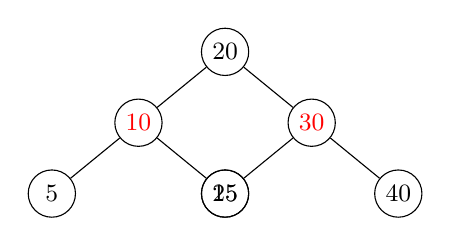
\begin{tikzpicture}[level distance=9mm, sibling distance=22mm,
    every node/.style={circle, draw, minimum size=6mm, inner sep=0pt, font=\small}]
    \node {20}
        child {node[text=red] {10}
            child {node {5}}
            child {node {15}}
        }
        child {node[text=red] {30}
            child {node {25}}
            child {node {40}}
        };
\end{tikzpicture}
\end{center}

Check each rule:
\begin{enumerate}[leftmargin=*]
    \item Every node colored -- yes.
    \item Root ($20$) is black -- yes.
    \item No red-red: $10$ and $30$ are red; their children ($5, 15, 25, 40$) are black -- OK.
    \item Nulls are black leaves -- by convention.
    \item Black-heights: from $20$ to any null sentinel under $5$, $15$, $25$, or $40$, we pass through $20, 5/15/25/40$, sentinel = 3 black nodes. Same on every path -- OK.
\end{enumerate}

All rules hold. Valid red-black tree.

\subsection*{Counterexample: a red-red violation}

\begin{center}
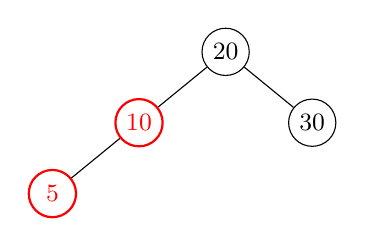
\begin{tikzpicture}[level distance=9mm, sibling distance=22mm,
    every node/.style={circle, draw, minimum size=6mm, inner sep=0pt, font=\small}]
    \node {20}
        child {node[text=red, draw=red, thick] {10}
            child {node[text=red, draw=red, thick] {5}} child[missing] {}
        }
        child {node {30}};
\end{tikzpicture}
\end{center}

Node $10$ is red, and its child $5$ is also red. Rule 3 violated. Not a valid red-black tree. Insertion or deletion code has to fix this kind of situation with recolorings and rotations -- that's what sections 9.6 and 9.7 will cover.

\subsection*{The bit-stealing trick}

In practice, the color bit is not stored as a separate byte. Every pointer on a modern architecture is 8-byte aligned, which means the low three bits of every node pointer are zero. Implementations ``steal'' one of those bits to encode color: \texttt{uintptr\_t(parent) | 1} means red, \texttt{uintptr\_t(parent) \& \textasciitilde 1} means black. Saves a full word per node and is standard technique in \texttt{std::\_Rb\_tree\_node}.

This isn't required for correctness -- you can use a \texttt{bool isRed} field -- but it shows how mature implementations pay zero storage overhead for the color state.

\begin{ideabox}
Red-black trees are a compromise: slightly looser balance invariant than AVL, but much more forgiving during rebalancing. The five rules look fiddly but are actually the minimal set that forces $O(\log n)$ height with the weakest possible constraints. AVL's ``differ by at most 1'' is tighter but more expensive to maintain. Red-black is the industry-standard choice because its looseness costs almost nothing in practice and its rebalancing code is (arguably) more tractable once you learn the cases.
\end{ideabox}

\subsection*{Looking ahead}

Section 9.6 will cover red-black \textbf{insertion}: attach a new node (always colored \emph{red} initially), then fix any red-red violation by recoloring or rotating. Section 9.7 will cover red-black \textbf{removal}: harder, because the deleted node's ``blackness'' can propagate upward as a ``double-black'' that needs careful resolution. Both operations end up with a small number of named cases -- six for insert, eight for delete -- which is why people find red-black trees intimidating. The good news: every case is a constant-work local fix.

\begin{warnbox}
Don't try to memorize the rules without understanding why they hold together. Rule 3 is the ``no clusters'' rule; rule 5 is the ``balanced depth'' rule; rules 1, 2, and 4 are administrative. If you forget a rule during a bug hunt, re-derive it: if rule 5 could be violated freely, a tree could be arbitrarily tall on one side with no compensating reds; if rule 3 could be violated, you could stack many reds along one path and bypass rule 5 trivially.
\end{warnbox}

\section{9.6 Red-Black Rotations}

Red-black rotations are \emph{the same operation} as AVL rotations: rewire three pointers to preserve BST ordering while reshaping a local subtree. The implementation differs only in what auxiliary state is maintained (color instead of height) and what triggers a rotation (a red-red violation or a black-height violation, not a $\pm 2$ balance factor).

This section states the primitives. Sections 9.7 uses them to implement red-black insert (and would cover remove).

\begin{defnbox}[Red-black rotation]
A rotation on a red-black tree is mechanically identical to an AVL rotation:
\begin{itemize}[leftmargin=*]
    \item \textbf{Left rotation at $X$} requires $X$'s right child to be non-null. $X$'s right child becomes the subtree's new root. (Colors are \emph{not} changed by the rotation itself -- they're a separate bookkeeping step.)
    \item \textbf{Right rotation at $X$} requires $X$'s left child to be non-null. Symmetric.
\end{itemize}
\end{defnbox}

No colors are rotated; they stay on their original nodes. This is subtle: in a rotation the node identities don't change, only the parent/child edges do. So if $X$ was red before a left rotation, $X$ is still red after; only its position in the tree moved.

\subsection*{Utility helpers}

The helper signatures mirror AVL's (section 9.2) minus the \texttt{avlUpdateHeight} call. Red-black doesn't cache a per-node height; it maintains color instead, which changes via explicit recolor operations (section 9.7), not automatically from structural changes.

\begin{lstlisting}
enum class Color { Red, Black };

template <typename T>
struct RBNode {
    T        data;
    Color    color  = Color::Red;      // new nodes default red (see 9.7)
    RBNode*  left   = nullptr;
    RBNode*  right  = nullptr;
    RBNode*  parent = nullptr;
};

template <typename T>
void rbSetChild(RBNode<T>* parent, bool isLeft, RBNode<T>* child) {
    if (isLeft) parent->left = child;
    else        parent->right = child;
    if (child != nullptr) child->parent = parent;
}

template <typename T>
void rbReplaceChild(RBNode<T>* parent,
                    RBNode<T>* currentChild,
                    RBNode<T>* newChild) {
    if (parent->left == currentChild)  rbSetChild(parent, true,  newChild);
    else                               rbSetChild(parent, false, newChild);
}
\end{lstlisting}

No height recomputation. No balance-factor check. Just pointer rewiring.

\subsection*{Left rotation algorithm}

\begin{lstlisting}
template <typename T>
void rbRotateLeft(RBNode<T>*& root, RBNode<T>* X) {
    RBNode<T>* Y  = X->right;        // must be non-null
    RBNode<T>* YL = Y->left;         // may be null

    if (X->parent != nullptr) rbReplaceChild(X->parent, X, Y);
    else                      { root = Y; Y->parent = nullptr; }

    rbSetChild(Y, true,  X);         // Y's left becomes X
    rbSetChild(X, false, YL);        // X's right becomes Y's old left
}
\end{lstlisting}

\subsection*{Right rotation algorithm}

The mirror image:

\begin{lstlisting}
template <typename T>
void rbRotateRight(RBNode<T>*& root, RBNode<T>* X) {
    RBNode<T>* Y  = X->left;         // must be non-null
    RBNode<T>* YR = Y->right;        // may be null

    if (X->parent != nullptr) rbReplaceChild(X->parent, X, Y);
    else                      { root = Y; Y->parent = nullptr; }

    rbSetChild(Y, false, X);
    rbSetChild(X, true,  YR);
}
\end{lstlisting}

\subsection*{Side-by-side with AVL rotation}

\begin{center}
\begin{tabular}{lll}
                         & AVL                         & Red-Black \\
\hline
Pointer rewires          & 3                           & 3 \\
Update cached field      & height(X), height(Y)        & none during rotate \\
Triggered by             & bf$(X) \in \{-2, +2\}$       & red-red or black-height violation \\
Preserves BST ordering   & yes                         & yes \\
Preserves balance        & no -- it \emph{fixes} balance & no -- it \emph{helps fix} balance along with recoloring \\
\end{tabular}
\end{center}

The shape-changing part is identical. Red-black's twist is that rotations alone don't restore the invariant -- you need \textbf{rotations + recolorings} together. Section 9.7 will show how those two primitives compose.

\subsection*{Example: a rotation as standalone visualization}

\begin{center}
Before left-rotate at $X$:
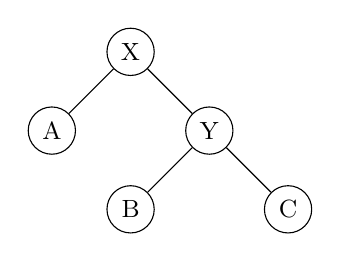
\begin{tikzpicture}[level distance=10mm, sibling distance=20mm,
    every node/.style={circle, draw, minimum size=6mm, inner sep=0pt, font=\small}]
    \node {X}
        child {node {A}}
        child {node {Y}
            child {node {B}}
            child {node {C}}
        };
\end{tikzpicture}
\quad $\to$ \quad
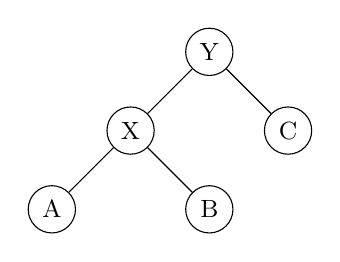
\begin{tikzpicture}[level distance=10mm, sibling distance=20mm,
    every node/.style={circle, draw, minimum size=6mm, inner sep=0pt, font=\small}]
    \node {Y}
        child {node {X}
            child {node {A}}
            child {node {B}}
        }
        child {node {C}};
\end{tikzpicture}
\end{center}

In-order sequence before: $A, X, B, Y, C$. After: $A, X, B, Y, C$. Identical. That's the invariant rotations preserve.

\subsection*{When rotations alone aren't enough}

A single rotation on a red-black tree typically \emph{does not} restore all five invariants. For example, a red node rotated to the top of a subtree might violate rule 2 (root must be black) or rule 3 (no red-red). That's why red-black insert and remove always combine rotations with explicit recoloring steps.

The cleanest way to think about it: rotations change \emph{structure}, recolorings change \emph{color state}, and the balanced-search-tree operations use both together to fix whatever rule was broken. Section 9.7 makes the dance explicit.

\begin{ideabox}
It's worth internalizing: every self-balancing BST ever invented (AVL, red-black, splay, weight-balanced, scapegoat, treap, AA-tree, 2-3-4 tree) uses rotations as its shape-changing primitive. The differences are only in the invariant being maintained and the trigger conditions for rotation. ``Rotations preserve BST ordering'' is the single fact you need to believe in; everything else is bookkeeping.
\end{ideabox}

\begin{warnbox}
Never conditionally skip a rotation ``because the tree looks OK.'' The insert/remove algorithms decide when to rotate based on the color configuration, not on eyeball balance. If you add a conditional like ``only rotate if the imbalance is large enough,'' you'll corrupt black-heights and the tree will silently stop being a valid red-black tree.
\end{warnbox}

\begin{notebox}
Production red-black implementations (the \texttt{std::map} backing tree, Java's \texttt{TreeMap}, Linux's \texttt{rbtree.c}) all use some variant of the helpers shown here. They inline the rotations into the insert/delete case code for speed, but the primitive is the same 3-pointer rewire with parent-pointer maintenance. Reading one production implementation once -- Linux's is the cleanest -- is one of the best ways to internalize the operations.
\end{notebox}

\section{9.7 Red-Black Insertion}

Red-black insertion has a reputation for being intimidating. The reputation is partially deserved -- there are more cases than in AVL -- but the logic breaks into a handful of symmetric pairs once you see the pattern. This section walks through the full algorithm and the five cases that can arise.

\begin{defnbox}[Red-black insert, high level]
\begin{enumerate}[leftmargin=*]
    \item \textbf{BST insert} the new node at the correct leaf position.
    \item \textbf{Color it red.} New nodes are always red initially. This preserves black-height (rule 5) but may create a red-red violation (rule 3) if the parent is also red.
    \item \textbf{Fix up} any red-red violation by recoloring and/or rotating. The fix-up walks from the new node toward the root, possibly recursing once per pair of levels.
\end{enumerate}
\end{defnbox}

\subsection*{Why color new nodes red?}

A color choice has to be made. If we colored new nodes black, rule 5 (equal black-height on every path) would immediately break -- the path through the new node now has one more black than the rest. Fixing that violation is hard; it cascades globally.

Red breaks only rule 3 (no red child of a red parent), and rule 3 is local -- you can see if it's violated by checking the new node's parent. If the parent is black, no violation, done. If the parent is red, local fix with one of five named cases. Much easier.

\subsection*{Terminology: parent, uncle, grandparent}

\begin{defnbox}[Family relationships]
For a node $n$:
\begin{itemize}[leftmargin=*]
    \item \textbf{Parent} = $n$'s parent.
    \item \textbf{Grandparent} = $n$'s parent's parent (may be null).
    \item \textbf{Uncle} = the grandparent's \emph{other} child -- the sibling of $n$'s parent (may be null).
\end{itemize}
The color of the uncle is the key discriminator in the insertion fix-up. A red uncle lets us ``push the violation up'' via recoloring; a black (or null) uncle requires a rotation.
\end{defnbox}

\begin{lstlisting}
template <typename T>
RBNode<T>* rbGrandparent(RBNode<T>* n) {
    return (n->parent != nullptr) ? n->parent->parent : nullptr;
}

template <typename T>
RBNode<T>* rbUncle(RBNode<T>* n) {
    RBNode<T>* g = rbGrandparent(n);
    if (g == nullptr) return nullptr;
    return (g->left == n->parent) ? g->right : g->left;
}
\end{lstlisting}

\subsection*{The five cases}

Let $n$ = the newly-inserted node, $p$ = $n$'s parent, $g$ = $n$'s grandparent, $u$ = $n$'s uncle.

\textbf{Case 1: $n$ is the root.} Just color it black. Done. (Rule 2.)

\textbf{Case 2: $p$ is black.} No red-red violation. Done.

\textbf{Case 3: $p$ is red and $u$ is red.} Recolor: $p$ and $u$ both become black, $g$ becomes red. Now black-heights are unchanged below $g$, but $g$ might now violate rule 3 with its own parent. \emph{Recursively apply fix-up to $g$.}

\textbf{Case 4: $p$ is red, $u$ is black (or null), $n$ is on the ``inside.''} \emph{Inside} means $n$ is a right child and $p$ is a left child, or vice versa. Rotate at $p$ to straighten the zig-zag into a zig-zig. Then fall through into case 5.

\textbf{Case 5: $p$ is red, $u$ is black (or null), $n$ is on the ``outside.''} \emph{Outside} means $n$ and $p$ are on the same side (both lefts, or both rights). Recolor $p$ black and $g$ red. Rotate at $g$ (right if $p$ was left, left if $p$ was right). Done.

The pattern: cases 3 and 5 recolor; cases 4 and 5 rotate; case 3 recurses; cases 4 and 5 terminate in $O(1)$.

\subsection*{Case 3 in detail: uncle is red}

\begin{center}
\emph{Before:} parent $P$ red, uncle $U$ red, grandparent $G$ black.
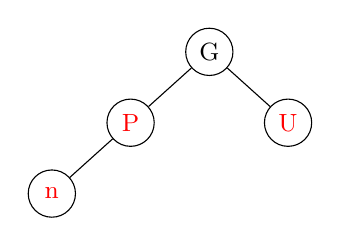
\begin{tikzpicture}[level distance=9mm, sibling distance=20mm,
    every node/.style={circle, draw, minimum size=6mm, inner sep=0pt, font=\small}]
    \node {G}
        child {node[text=red] {P}
            child {node[text=red] {n}}
            child[missing] {}
        }
        child {node[text=red] {U}};
\end{tikzpicture}
\quad $\to$ \quad
\emph{After recolor:}
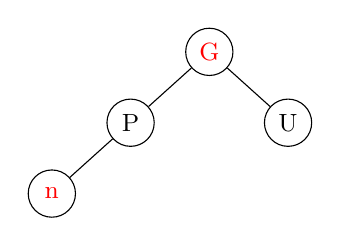
\begin{tikzpicture}[level distance=9mm, sibling distance=20mm,
    every node/.style={circle, draw, minimum size=6mm, inner sep=0pt, font=\small}]
    \node[text=red] {G}
        child {node {P}
            child {node[text=red] {n}}
            child[missing] {}
        }
        child {node {U}};
\end{tikzpicture}
\end{center}

No structure changed; only colors. But $G$ is now red, which may conflict with $G$'s parent. Recurse the fix-up on $G$. Black-height from any ancestor of $G$ is preserved because $G$'s path had one black (itself) replaced by a red (itself) but both paths through $P$ and $U$ gained a black (those nodes became black), so the net along every path stayed the same.

\subsection*{Cases 4 and 5: uncle is black}

This is where rotations come in. If the uncle is black, recoloring alone would break rule 5 -- the uncle's path was already black-height balanced, and changing colors without a rotation would shift the count.

\textbf{Case 4 (zig-zag $\to$ zig-zig):} suppose $n$ is the right child of $p$, and $p$ is the left child of $g$. Left-rotate at $p$; this swings $n$ into $p$'s old position with $p$ as $n$'s left child. Now $n$ and its new left child ($p$) are both ``on the left'' of $g$ -- we've transformed into case 5. Relabel: what was ``$n$'' we now call ``$p$,'' and fall through.

\begin{center}
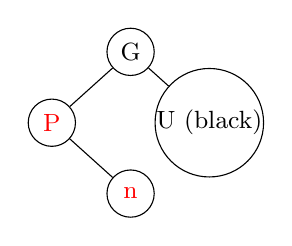
\begin{tikzpicture}[level distance=9mm, sibling distance=20mm,
    every node/.style={circle, draw, minimum size=6mm, inner sep=0pt, font=\small}]
    \node {G}
        child {node[text=red] {P}
            child[missing] {}
            child {node[text=red] {n}}
        }
        child {node {U (black)}};
\end{tikzpicture}
\quad $\to$ \quad
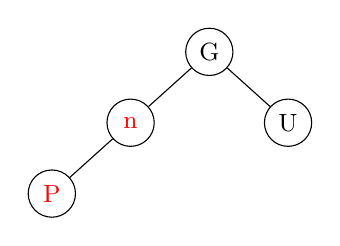
\begin{tikzpicture}[level distance=9mm, sibling distance=20mm,
    every node/.style={circle, draw, minimum size=6mm, inner sep=0pt, font=\small}]
    \node {G}
        child {node[text=red] {n}
            child {node[text=red] {P}}
            child[missing] {}
        }
        child {node {U}};
\end{tikzpicture}
\end{center}

Now apply case 5.

\textbf{Case 5 (zig-zig $\to$ fixed):} Recolor $P$ black, $G$ red, then rotate right at $G$:

\begin{center}
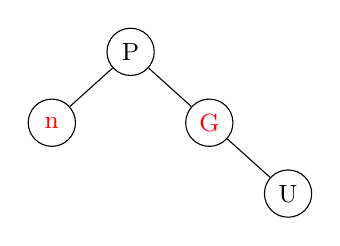
\begin{tikzpicture}[level distance=9mm, sibling distance=20mm,
    every node/.style={circle, draw, minimum size=6mm, inner sep=0pt, font=\small}]
    \node {P}
        child {node[text=red] {n}}
        child {node[text=red] {G}
            child[missing] {}
            child {node {U}}
        };
\end{tikzpicture}
\end{center}

Now $P$ is black (satisfies root or whatever parent $G$ had), $n$ and $G$ are red (but neither has a red parent), and the black-height through every path is the same as before the insertion. Done in $O(1)$.

\subsection*{The full fix-up loop}

\begin{lstlisting}
template <typename T>
void rbBalance(RBNode<T>*& root, RBNode<T>* n) {
    while (true) {
        if (n->parent == nullptr) {             // case 1: n is root
            n->color = Color::Black;
            return;
        }
        if (n->parent->color == Color::Black)   // case 2
            return;

        RBNode<T>* p = n->parent;
        RBNode<T>* g = rbGrandparent(n);
        RBNode<T>* u = rbUncle(n);

        if (u != nullptr && u->color == Color::Red) {  // case 3
            p->color = Color::Black;
            u->color = Color::Black;
            g->color = Color::Red;
            n = g;                              // recurse upward
            continue;
        }

        // Cases 4/5: uncle is black (or null).
        // Case 4: straighten zig-zag into zig-zig.
        if (n == p->right && p == g->left) {
            rbRotateLeft(root, p);
            n = n->left;                        // which is the old p
        } else if (n == p->left && p == g->right) {
            rbRotateRight(root, p);
            n = n->right;                       // which is the old p
        }

        // Case 5: zig-zig fix.
        p = n->parent;
        g = rbGrandparent(n);
        p->color = Color::Black;
        g->color = Color::Red;
        if (n == p->left) rbRotateRight(root, g);
        else              rbRotateLeft(root, g);
        return;                                 // O(1) termination
    }
}

template <typename T>
void rbInsert(RBNode<T>*& root, RBNode<T>* node) {
    // Phase 1: BST insert. (Identical to chapter 6 insert; omitted.)
    bstInsert(root, node);
    node->color = Color::Red;
    rbBalance(root, node);
}
\end{lstlisting}

\subsection*{Cost}

\begin{center}
\begin{tabular}{ll}
Phase & Cost \\
\hline
BST descent              & $O(\log n)$ \\
Fix-up loop              & $O(\log n)$ iterations in the worst case (case 3 recurses) \\
Rotations per insertion  & At most 2 (from case 4/5, one shot) \\
Recolorings per insertion & Up to $O(\log n)$ (case 3 cascade) \\
\hline
\textbf{Total}           & $\mathbf{O(\log n)}$ \\
\end{tabular}
\end{center}

Insert is always $O(\log n)$ and -- notably -- does at most \emph{two} rotations, regardless of how many recolorings happen. That low rotation count (compared to AVL's worst case) is part of why red-black is preferred in practice: rotations are more expensive than recolorings (three pointer writes vs.\ one bit flip), and capping rotations at 2 per insert is a solid guarantee.

\begin{ideabox}
The case-3 recursion is ``the violation walks up the tree'' -- each level is fixed by demoting the grandparent to red, which may re-create a red-red with great-grandparent, and so on. But each step only touches three nodes' colors; no rotations yet. Only when we hit a black uncle do we commit to a rotation, and that rotation terminates the whole cascade. The recoloring is the workhorse; the rotations are the cleanup.
\end{ideabox}

\subsection*{A worked insertion sequence}

Start empty. Insert 22, 11, 33, 55, 44:

\begin{itemize}[leftmargin=*]
    \item \texttt{insert(22)}: root, colored black. Tree: \{22(B)\}.
    \item \texttt{insert(11)}: BST puts it left of 22, colored red. Parent black, case 2. Tree: \{22(B), 11(R)\}.
    \item \texttt{insert(33)}: right of 22, red. Parent black, case 2. Tree: \{22(B), 11(R), 33(R)\}.
    \item \texttt{insert(55)}: right of 33, red. Parent 33 is red, uncle 11 is red -- case 3. Recolor: 11(B), 33(B), 22(R). Recurse at 22. 22 is root, case 1 forces it back to black. Tree: \{22(B), 11(B), 33(B), 55(R)\}.
    \item \texttt{insert(44)}: left of 55, red. Parent 55 red, uncle = right child of 33 = null (black). 44 is left child of 55, 55 is right child of 33 -- case 4 (zig-zag). Right-rotate at 55: 44 becomes 33's right child, 55 becomes 44's right child. Then case 5: recolor 44(B), 33(R). Left-rotate at 33. Done.
\end{itemize}

The whole sequence involves one cascading recolor and one case-4-plus-5 double-rotation. Total for five insertions: at most 2 rotations and a handful of color flips. Tree stays $O(\log n)$ tall throughout.

\begin{warnbox}
Case 4 and case 5 are \emph{sequential}, not alternatives. Case 4 transforms the imbalance into a shape that case 5 can finish. Don't write them as an \texttt{if/else} that picks one or the other -- write case 4 as a precondition transform that falls through into case 5. The loop structure should be ``optionally do case 4, then always do case 5.''
\end{warnbox}

\begin{examplebox}
\textbf{Worked red-black insertion: $10, 20, 30, 40, 50, 25$ (same
input as the AVL examplebox in \S9.3).} Reading both traces
side-by-side is pedagogically powerful: same input, different
machinery, both maintain $h = O(\log n)$. We show the colour state
after each insert plus the cases that fire. ``B'' = black, ``R'' =
red.

\textbf{Frame 1 -- insert $10$.} New root. Coloured red on entry,
then case 1 (root) recolours to black.
\[
10\,\text{B}
\]

\textbf{Frame 2 -- insert $20$.} BST puts $20$ to right of $10$;
new node coloured red. Parent ($10$) is black: \textbf{case 2}, no
fix-up.
\[
10\,\text{B},\,\, \text{right} = 20\,\text{R}
\]

\textbf{Frame 3 -- insert $30$.} BST descends right of $10$, right
of $20$; new node red. Parent ($20$) is red, uncle ($10$'s left
child) is null $\Rightarrow$ treated as black; $30$ is the
\emph{outside} grandchild (right of $20$, $20$ is right of $10$):
\textbf{case 5} (zig-zig). Recolour: $20$ B, $10$ R; left-rotate at
$10$.
\[
20\,\text{B},\,\, \text{left} = 10\,\text{R},\,\, \text{right} = 30\,\text{R}
\]

\textbf{Frame 4 -- insert $40$.} BST: right of $30$; red. Parent
($30$) is red, uncle ($10$, left of $20$) is red $\Rightarrow$
\textbf{case 3}. Recolour $30$ B, $10$ B, $20$ R. Recurse on $20$:
$20$ is the root, case 1 forces it back to black.
\[
20\,\text{B},\,\, 10\,\text{B},\,\, 30\,\text{B},\,\, 40\,\text{R}
\]

\textbf{Frame 5 -- insert $50$.} BST: right of $40$; red. Parent
($40$) is red, uncle ($30$'s left = null = black);
\emph{outside} grandchild (right of $40$, $40$ is right of $30$):
\textbf{case 5}. Recolour $40$ B, $30$ R; left-rotate at $30$.
$40$ is now $20$'s right child with $30$ R left, $50$ R right.
Re-check: parent ($20$) is black, no further fix-up.
\[
\begin{array}{l}
20\,\text{B} \\
\quad \text{left}: 10\,\text{B} \\
\quad \text{right}: 40\,\text{B} \\
\qquad \text{left}: 30\,\text{R},\,\, \text{right}: 50\,\text{R}
\end{array}
\]

\textbf{Frame 6 -- insert $25$.} BST descent: right of $20$, left
of $40$, left of $30$; new node red. Parent ($30$) is red, uncle
($50$) is red $\Rightarrow$ \textbf{case 3}. Recolour $30$ B,
$50$ B, $40$ R. Recurse on $40$. $40$'s parent ($20$) is black:
case 2, terminate.
\[
\begin{array}{l}
20\,\text{B} \\
\quad \text{left}: 10\,\text{B} \\
\quad \text{right}: 40\,\text{R} \\
\qquad \text{left}: 30\,\text{B} \\
\qquad\quad \text{left}: 25\,\text{R} \\
\qquad \text{right}: 50\,\text{B}
\end{array}
\]
Verify the invariant: black-height from $20$ to any null leaf is
$3$ on every path (count: $20, 30/50, $ null $\,= 3$ via
$30$/$50$; $20, 10, $ null $ = 3$ via $10$; $20, 40$ red, $30$ B,
$25$ R, null = $3$ blacks). All paths balance.

\textbf{Takeaway.} Six inserts produced \emph{two} case-3
recolouring cascades and \emph{two} case-5 single-rotation fixes
(no case-4 zig-zag triggered, because none of the inserts landed
on an ``inside'' grandchild with a black uncle). Compare to the
AVL trace: AVL needed three rotations (one of which was a
\emph{double} rotation); red-black needed two single rotations
plus four colour flips. The case-3 recurse-on-grandparent step on
inserts $40$ and $25$ is the source of the $O(\log n)$ recolouring
worst case; the rotations cap at two regardless. \emph{This is
why \texttt{std::map} chose red-black: rotations are pointer
writes, recolours are bit flips.}
\end{examplebox}

\begin{notebox}
Red-black \emph{removal} follows the same spirit -- BST remove first, then fix any invariant violation -- but with more cases because removing a black node breaks rule 5 directly. That's the subject of the next section.
\end{notebox}

\section{9.8 Red-Black Tree: Removal}

Red-black removal is the most intricate operation in any red-black implementation. Insertion has five cases, rotations are a few lines -- removal has six named cases on top of the BST removal logic. This section walks through all of it, but keep the big picture in mind while the details fly by:

\begin{ideabox}
\textbf{The whole removal story, one paragraph.}
\begin{enumerate}[leftmargin=*]
    \item BST-remove the node. But first, if it's internal, swap with its predecessor so we're always deleting a node with at most one child.
    \item Removing a \emph{red} node is free -- black-heights don't change, no rule is violated. Done.
    \item Removing a \emph{black} node drops the black count along one path by 1, violating rule 5 (equal black-heights). We have to fix this \emph{before} we remove the node.
    \item The fix is a cascade of six cases that massage the tree so the node becomes removable without violating any invariant -- sometimes by recoloring, sometimes by rotating, sometimes by pushing the problem one level up.
\end{enumerate}
\end{ideabox}

\subsection*{Step 1: High-level remove}

The entry point is \texttt{rbRemove(tree, key)}, which is just BST search + dispatch to node-removal:

\begin{lstlisting}[basicstyle=\ttfamily\small,frame=single]
void rbRemove(RBTree& t, int key) {
    RBNode* n = bstSearch(t.root, key);
    if (n) rbRemoveNode(t, n);
}
\end{lstlisting}

\texttt{rbRemoveNode} handles the classic BST ``two-children'' reduction: if \texttt{n} has both children, copy the predecessor's key into \texttt{n} and recursively remove the predecessor node instead. Predecessors are leaves or have only a left child, so we always end up removing a node with $\leq 1$ child:

\begin{lstlisting}[basicstyle=\ttfamily\small,frame=single]
void rbRemoveNode(RBTree& t, RBNode* n) {
    if (n->left && n->right) {
        RBNode* pred = rbPredecessor(n);
        int predKey = pred->key;
        rbRemoveNode(t, pred);   // recurse on a <= 1-child node
        n->key = predKey;
        return;
    }
    if (n->color == Color::Black)
        rbPrepareForRemoval(t, n);   // fix black-height BEFORE removing
    bstRemove(t, n->key);            // ordinary BST splice-out
}

RBNode* rbPredecessor(RBNode* n) {
    n = n->left;
    while (n->right) n = n->right;
    return n;
}
\end{lstlisting}

\begin{warnbox}
\textbf{Order matters.} \texttt{rbPrepareForRemoval} runs \emph{before} \texttt{bstRemove}. We want to rebalance while the tree still has \texttt{n} in place, so we can identify its sibling, parent, and nephews. After the BST splice, that context is gone.
\end{warnbox}

\subsection*{Why red is easy, black is hard}

Removing a node means splicing out \texttt{n} and replacing it with its (single or null) child. Two rules could break:

\begin{itemize}[leftmargin=*]
    \item \textbf{Rule 3 (no two reds in a row).} Removing a node can't \emph{create} a red-red pair as long as we replace with the correct child. Insertion worries about this; removal doesn't.
    \item \textbf{Rule 5 (equal black-heights).} Every root-to-null path must have the same count of black nodes. Removing a \emph{black} node decrements that count along one path.
\end{itemize}

If \texttt{n} is red, the black count doesn't change, and rule 3 is safe because \texttt{n}'s child must have been black (rule 3). Nothing to do.

If \texttt{n} is black, rule 5 breaks. Classical textbooks solve this by imagining \texttt{n}'s replacement carries an extra ``double-black'' token, and the fix-up pushes that token around until it reaches the root or cancels against a red. The textbook here takes an equivalent but more operational view: classify the local neighborhood into six cases and rewrite it until removal is safe.

\subsection*{Utility functions}

Four helpers make the case logic readable. Critically, \textbf{a null pointer counts as a black node} in all of them -- matching rule 2 (null leaves are black):

\begin{lstlisting}[basicstyle=\ttfamily\small,frame=single]
RBNode* rbSibling(RBNode* n) {
    if (!n->parent) return nullptr;
    return (n == n->parent->left) ? n->parent->right : n->parent->left;
}

bool rbIsRed(RBNode* n) {
    return n && n->color == Color::Red;
}

bool rbIsBlack(RBNode* n) {
    return !n || n->color == Color::Black;   // null is black
}

bool rbBothChildrenBlack(RBNode* n) {
    return rbIsBlack(n->left) && rbIsBlack(n->right);
}
\end{lstlisting}

\subsection*{Step 2: Prepare-for-removal, the six cases}

The prepare-for-removal routine classifies the local neighborhood of \texttt{n} (its color, parent, sibling, and sibling's children) and applies one of six rewrites. Cases 1, 3, 4 are terminal -- once they fire, prep is done. Cases 2, 5, 6 are \emph{transitional} -- they massage the tree and fall through to later cases.

\begin{examplebox}
\textbf{What each case is really trying to do.}
\begin{itemize}[leftmargin=*]
    \item \textbf{Case 1} ``We're already OK.'' Node is red, or we're at the root -- nothing to fix.
    \item \textbf{Case 2} ``Sibling is red -- make it black first.'' Rotate to put a black sibling in place so cases 3--6 can run.
    \item \textbf{Case 3} ``Whole neighborhood is black -- push the deficit up.'' Recolor sibling red, recurse on the parent. The subtree is now internally balanced, but the parent has lost a black from above; that's the parent's problem now.
    \item \textbf{Case 4} ``Parent is red, sibling branch is all black -- swap colors locally.'' Swap parent's red to sibling, parent becomes black. Done in $O(1)$.
    \item \textbf{Case 5} ``Zig-zag sibling -- straighten it.'' Rotate on the sibling so we can finish with case 6's big rotation.
    \item \textbf{Case 6} ``Final rotation.'' Rotate at the parent, recolor. This is where the deficit is permanently absorbed.
\end{itemize}
\end{examplebox}

\subsubsection*{The driver}

\begin{lstlisting}[basicstyle=\ttfamily\small,frame=single]
void rbPrepareForRemoval(RBTree& t, RBNode* n) {
    if (rbTryCase1(n)) return;

    RBNode* s = rbSibling(n);
    if (rbTryCase2(t, n, s)) s = rbSibling(n);
    if (rbTryCase3(t, n, s)) return;
    if (rbTryCase4(n, s))    return;
    if (rbTryCase5(t, n, s)) s = rbSibling(n);
    if (rbTryCase6(t, n, s)) s = rbSibling(n);

    // Fall-through: the final rotation (always runs if we got here).
    s->color = n->parent->color;
    n->parent->color = Color::Black;
    if (n == n->parent->left) {
        s->right->color = Color::Black;
        rbRotateLeft(t, n->parent);
    } else {
        s->left->color = Color::Black;
        rbRotateRight(t, n->parent);
    }
}
\end{lstlisting}

Note the structure: after case 2, the sibling may have changed (it rotated out), so we refetch. Same after cases 5 and 6. Cases 3 and 4 \texttt{return} immediately. Cases 5 and 6 \emph{prepare} the configuration for the final fall-through rotation.

\subsubsection*{Case 1 -- trivially removable}

\begin{lstlisting}[basicstyle=\ttfamily\small,frame=single]
bool rbTryCase1(RBNode* n) {
    return (n->color == Color::Red) || (n->parent == nullptr);
}
\end{lstlisting}

A red node's removal doesn't disturb black-heights. A root node's removal -- after the BST splice reduces it to a trivial case -- is also fine (any single remaining child becomes the new root, will be recolored black implicitly by the fix-up of its children). No action required.

\subsubsection*{Case 2 -- red sibling}

\begin{lstlisting}[basicstyle=\ttfamily\small,frame=single]
bool rbTryCase2(RBTree& t, RBNode* n, RBNode* s) {
    if (!rbIsRed(s)) return false;
    n->parent->color = Color::Red;
    s->color = Color::Black;
    if (n == n->parent->left) rbRotateLeft(t, n->parent);
    else                      rbRotateRight(t, n->parent);
    return true;
}
\end{lstlisting}

If the sibling is red, the parent must be black (rule 3), and the sibling's two children must be black (rule 3 again). Rotate at the parent to promote the sibling up, recolor so the old parent is red and the old sibling is black. \texttt{n} now has a \emph{black} sibling (which is one of the former sibling's children) -- that's the precondition for cases 3--6, which do the real work.

\begin{notebox}
Case 2 doesn't solve anything by itself -- it normalizes the tree so the harder cases can match. That's why it falls through.
\end{notebox}

\subsubsection*{Case 3 -- push the deficit up}

\begin{lstlisting}[basicstyle=\ttfamily\small,frame=single]
bool rbTryCase3(RBTree& t, RBNode* n, RBNode* s) {
    if (n->parent->color != Color::Black) return false;
    if (!rbBothChildrenBlack(s))          return false;
    s->color = Color::Red;
    rbPrepareForRemoval(t, n->parent);   // recurse one level up
    return true;
}
\end{lstlisting}

Parent black, sibling black, sibling's children black. Recolor the sibling red -- that drops the black count on the sibling's side by 1, matching the drop we're about to cause on \texttt{n}'s side. Now the subtree rooted at the parent has consistent black-heights internally, but the parent as a whole has \emph{one fewer black} on all paths through it than before. That's the same problem we started with, one level higher -- so we recurse on the parent.

\begin{ideabox}
Case 3 is where the $O(\log n)$ cost of removal comes from. The other cases are constant-time terminal fixes; only case 3 can chain up the tree, and it runs at most $h = O(\log n)$ times before hitting the root (case 1).
\end{ideabox}

\subsubsection*{Case 4 -- swap colors}

\begin{lstlisting}[basicstyle=\ttfamily\small,frame=single]
bool rbTryCase4(RBNode* n, RBNode* s) {
    if (n->parent->color != Color::Red) return false;
    if (!rbBothChildrenBlack(s))        return false;
    n->parent->color = Color::Black;
    s->color = Color::Red;
    return true;
}
\end{lstlisting}

Parent red, sibling branch all black. Swap: parent becomes black, sibling becomes red. On \texttt{n}'s path, we lose a black (from removing \texttt{n}) but gain one (parent flipped to black) -- net zero. On the sibling's path, we lose one (sibling flipped to red) but gain one (parent flipped to black) -- net zero. Rule 3 holds because the sibling's children were already black. Done.

\subsubsection*{Case 5 -- straighten zig-zag (mirror of insertion case 4)}

\begin{lstlisting}[basicstyle=\ttfamily\small,frame=single]
bool rbTryCase5(RBTree& t, RBNode* n, RBNode* s) {
    if (!rbIsRed(s->left))             return false;
    if (!rbIsBlack(s->right))          return false;
    if (n != n->parent->left)          return false;
    s->color = Color::Red;
    s->left->color = Color::Black;
    rbRotateRight(t, s);
    return true;
}
\end{lstlisting}

This preps for case 6. If \texttt{n} is a left child and the sibling's ``outer'' child (sibling's right) is black while its ``inner'' child is red, a rotation at the sibling moves the red to the outer position -- now case 6 (or the fall-through) can do its single final rotation.

\subsubsection*{Case 6 -- mirror of case 5}

\begin{lstlisting}[basicstyle=\ttfamily\small,frame=single]
bool rbTryCase6(RBTree& t, RBNode* n, RBNode* s) {
    if (!rbIsBlack(s->left))           return false;
    if (!rbIsRed(s->right))            return false;
    if (n != n->parent->right)         return false;
    s->color = Color::Red;
    s->right->color = Color::Black;
    rbRotateLeft(t, s);
    return true;
}
\end{lstlisting}

Same as case 5 but for when \texttt{n} is a right child. Prepares for the fall-through rotation.

\subsubsection*{The fall-through rotation}

After case 5 or 6 (or if neither applied), the sibling has a red child in the ``outer'' position. The driver's tail runs:

\begin{itemize}[leftmargin=*]
    \item Sibling inherits the parent's color.
    \item Parent becomes black.
    \item The outer red child of the sibling becomes black.
    \item Rotate at the parent (left if \texttt{n} was left child, right otherwise).
\end{itemize}

The effect: the sibling becomes the new subtree root, painted the old parent's color (so external black count is preserved). The parent goes down to \texttt{n}'s side, now black (compensating for \texttt{n}'s upcoming removal). The sibling's outer red child goes to the opposite side, now black (compensating for the shift on that side). All black-heights are restored -- and \texttt{n} can now be BST-removed without any violation.

\subsection*{Why this many cases?}

\begin{ideabox}
Red-black removal has six cases because the local neighborhood can be in six structurally distinct shapes, each needing a different rewrite to restore rule 5 without breaking rule 3. Insertion had only five cases because the only inserted node is always red and always a leaf -- removal has to cope with arbitrary existing structure around the deletion point.
\end{ideabox}

\begin{warnbox}
\textbf{The textbook treatment varies.} CLRS presents the same algorithm as four cases by merging symmetric pairs; the presentation here splits the fall-through rotation into two steps (cases 5/6 + the tail) where CLRS fuses them. The operations are identical; only the bookkeeping differs. If you cross-reference another source, expect the case numbering to shift.
\end{warnbox}

\subsection*{Cost analysis}

\begin{itemize}[leftmargin=*]
    \item \textbf{Find the node}: $O(\log n)$ BST search.
    \item \textbf{Two-children reduction}: at most one recursive descent to the predecessor, another $O(\log n)$.
    \item \textbf{Prepare-for-removal}: at most 3 rotations (case 2 + case 5 + fall-through, or case 2 + case 6 + fall-through). Case 3 can recurse up the tree $O(\log n)$ times, but each iteration is $O(1)$ recoloring. So the total fix-up work is $O(\log n)$.
    \item \textbf{Total}: $O(\log n)$ time, $O(\log n)$ stack depth (can be rewritten iteratively with parent pointers).
\end{itemize}

\begin{notebox}
\textbf{AVL vs.\ red-black removal.} AVL removal can cascade up to $O(\log n)$ rotations; red-black removal does at most 3 rotations (the rest is just recoloring). That's the classic reason \texttt{std::map} chose red-black: insertion/removal are both cheaper in rotation count, and rotations involve actual pointer writes, while recoloring is just a bit flip. For workloads heavy on modifications, the constant-factor win matters.
\end{notebox}

\subsection*{Putting it all together}

The complete removal interface:

\begin{lstlisting}[basicstyle=\ttfamily\small,frame=single]
void rbRemove(RBTree& t, int key) {
    RBNode* n = bstSearch(t.root, key);
    if (n) rbRemoveNode(t, n);
}

void rbRemoveNode(RBTree& t, RBNode* n) {
    if (n->left && n->right) {
        RBNode* pred = rbPredecessor(n);
        int k = pred->key;
        rbRemoveNode(t, pred);
        n->key = k;
        return;
    }
    if (n->color == Color::Black)
        rbPrepareForRemoval(t, n);
    bstRemove(t, n->key);
}
\end{lstlisting}

\begin{examplebox}
\textbf{Worked red-black removal traces.} A single small tree
doesn't exercise all four CLRS \texttt{RB-DELETE-FIXUP} cases (which
this chapter splits into six -- see the warnbox above), so we run
two short traces. ``B'' = black, ``R'' = red, double-black is
written ``DB'' for the conceptual deficit token.

\textbf{Trace A -- delete $50$ from a 7-node tree (case 1 + case 4).}
Start:
\[
\begin{array}{l}
30\,\text{B} \\
\quad \text{left}: 20\,\text{B} \\
\qquad \text{left}: 10\,\text{R} \\
\quad \text{right}: 50\,\text{B} \\
\qquad \text{left}: 40\,\text{R},\,\, \text{right}: 60\,\text{R}
\end{array}
\]
\texttt{rbRemoveNode} sees $50$ has two children, swaps with
predecessor ($40$), and recurses on $40$. $40$ is red $\Rightarrow$
\textbf{case 1} (trivially removable): no prep needed,
\texttt{bstRemove} just splices $40$ out.
\[
\begin{array}{l}
30\,\text{B} \\
\quad \text{left}: 20\,\text{B} \to 10\,\text{R} \\
\quad \text{right}: 40\,\text{B}\,\, (\text{key copied from old } 50) \\
\qquad \text{right}: 60\,\text{R}
\end{array}
\]
Now delete $40$ (which is now black, root's right child).
$40$'s sibling is $20$ (black); $20$'s children are $10$ R and
null (black). Sibling is black, parent ($30$) is black, sibling's
children are mixed -- not all black -- so case 3 doesn't fire.
The fall-through path applies: re-examine. Actually: parent
\emph{black}, sibling \emph{black}, sibling has at least one red
child ($10$). $40$ is the right child of $30$, sibling's
\emph{outer} child (left of $20$, when $40$ is on the right) is
$10$ R. Falls through to the tail rotation. Sibling ($20$)
inherits parent's colour (black), parent goes black (already),
the outer red ($10$) goes black, right-rotate at $30$. Final:
\[
\begin{array}{l}
20\,\text{B} \\
\quad \text{left}: 10\,\text{B} \\
\quad \text{right}: 30\,\text{B},\,\, \text{right} = 60\,\text{R}
\end{array}
\]
Black-height $= 2$ on every path. Done.

\textbf{Trace B -- delete $1$ from a 6-node tree (case 3 cascade).}
Start (constructed to force a case-3 propagation):
\[
\begin{array}{l}
20\,\text{B} \\
\quad \text{left}: 10\,\text{B} \\
\qquad \text{left}: 1\,\text{B},\,\, \text{right}: 15\,\text{B} \\
\quad \text{right}: 30\,\text{B} \\
\qquad \text{right}: 40\,\text{R}
\end{array}
\]
Delete $1$. $1$ is a black leaf, sibling $15$ is black with both
children null (black), parent $10$ is black, $1$'s removal would
drop black-count by 1 on its path $\Rightarrow$ \textbf{case 3}:
recolour sibling $15$ red, recurse on parent $10$. Now treat $10$
as the deficit-bearer.

At $10$: its sibling is $30$ (black), $30$'s children are null
(black) and $40$ R. Parent ($20$) is black; sibling has at least
one red child. So case 3 doesn't apply at this level; it's a
standard sibling-with-red-nephew configuration. $10$ is the
\emph{left} child of $20$; sibling's \emph{outer} child (right of
$30$) is $40$ R $\Rightarrow$ fall-through tail rotation
(equivalently CLRS case 4). Sibling ($30$) inherits parent's
colour (black), parent goes black, outer red ($40$) goes black,
left-rotate at $20$. Combined with the case-3 recolour and the
actual splice of $1$:
\[
\begin{array}{l}
30\,\text{B} \\
\quad \text{left}: 20\,\text{B} \\
\qquad \text{left}: 10\,\text{B},\,\, \text{right}: 15\,\text{R}\,(\text{(was sibling, recoloured in case 3)}) \\
\qquad\quad \text{(}10\text{'s left, where }1\text{ was, now null)} \\
\quad \text{right}: 40\,\text{B}
\end{array}
\]
Black-height $= 2$ on every path. Done.

\textbf{Cases exercised.} Trace A covered \emph{case 1}
(red node, trivial) and the \emph{fall-through tail rotation}
(equivalent to CLRS case 4). Trace B covered \emph{case 3}
(black-everywhere recurse) plus the same fall-through. The
remaining cases (\emph{case 2} red sibling, the explicit
\emph{case 5/6} zig-zag straighten) require slightly different
starting shapes -- the gap-report tradeoff was worked traces
covering as many cases as two compact trees allow rather than
one synthetic mega-example. The driver code in
\texttt{rbPrepareForRemoval} above runs every case in the same
way it ran here: classify, rewrite, re-classify if transitional,
fall through to the rotation tail when prep is complete.
\end{examplebox}

\begin{ideabox}
\textbf{The mental model to keep -- and where the rest of the book
takes you.} A red-black tree is a BST with bookkeeping. Every
modifying operation is (1) do the BST thing, (2) fix the
coloring/height invariants locally, (3) if local fix is impossible,
propagate one level up. Insertion propagates up with
\emph{uncle-red} recoloring; removal propagates up with
\emph{case 3} recoloring. Both walk at most $O(\log n)$ levels,
bounded by the tree height, which rule 5 guarantees is
$O(\log n)$.

\medskip

\textbf{Looking ahead.} Three forward references close the loop:
\begin{itemize}[leftmargin=*]
    \item \textbf{Chapter 10 (graphs).} BFS spanning trees and
          Dijkstra's parent-pointer trees are a different
          ``tree as algorithm output'' lens -- the tree isn't the
          data structure, it's the trace of a search. But the
          \emph{priority queue} that drives Dijkstra and Prim is
          often a balanced BST under the hood (Linux kernel CFS
          uses red-black trees for exactly this) -- so AVL/RB
          show up again on the inside of those algorithms.
    \item \textbf{Chapter 11 (B-trees).} The
          \emph{shallow-and-wide} alternative: same balanced search
          tree problem, different geometric tradeoff. AVL/RB are
          binary; B-trees fan out by hundreds per node. Same
          $O(\log n)$ asymptotic, but with cache-line and
          disk-page locality that this chapter's binary trees
          can't match. The augmentation framework from \S9.9
          carries over -- B-trees augment with key-counts and
          sometimes interval bounds.
    \item \textbf{Chapter 12 (set ADT).} The \emph{abstraction/
          implementation} closure. \texttt{std::set} and
          \texttt{std::map} are red-black trees under the hood --
          chapter 12 covers the interface and the standard library
          API; this chapter covered the implementation. Reading
          \texttt{libstdc++}'s \texttt{\_Rb\_tree.h} after this
          chapter is the practitioner-level capstone exercise.
\end{itemize}
\end{ideabox}

\section{9.9 Augmenting balanced trees}

\S9.4's framing notebox hinted at it; this section makes it
explicit. The \emph{cached height} trick that powers AVL
rebalancing is one example of a much more general pattern: a
balanced BST is a substrate on which you can attach a per-subtree
property and maintain it for free. Once you see the pattern, every
specialised balanced tree (order-statistic trees, interval trees,
range-sum trees) becomes ``a balanced BST with one more cached
field per node, plus an updated rotation routine.''

\begin{defnbox}[Subtree augmentation framework]
A \textbf{subtree augmentation} of a balanced BST is a property
$P$ defined at every node such that:
\begin{enumerate}[leftmargin=*]
    \item \textbf{Subtree-summarising.} $P(n)$ is a function of $n$
          and the subtree rooted at $n$. Examples: the height of
          $n$'s subtree (AVL); the number of nodes in $n$'s
          subtree (order-statistic); the maximum interval-endpoint
          stored in $n$'s subtree (interval tree).
    \item \textbf{$O(1)$ recomputable from children.} Given $P$
          values stored at $n$'s left and right children, $P(n)$
          can be computed in $O(1)$ from those two values plus
          $n$'s own data.
\end{enumerate}
Properties satisfying both clauses are maintained at zero
asymptotic overhead per insert/delete, because the existing
$O(\log n)$ retrace already touches every ancestor on the modified
path; recomputing $P$ at each touched ancestor is $O(1)$ per
ancestor, totalling $O(\log n)$ per operation -- the same
asymptotic as the operation itself.
\end{defnbox}

\subsection*{Worked example: subtree size for order-statistic queries}

The canonical example is \textbf{order-statistic trees} (CLRS
\S14.1). We want two new operations on a balanced BST:
\begin{itemize}[leftmargin=*]
    \item \texttt{select(k)} -- return the $k$-th smallest key,
          $0$-indexed.
    \item \texttt{rank(x)} -- return the number of keys strictly
          less than $x$.
\end{itemize}
Both run in $O(\log n)$ with the right augmentation. The augmented
property is $P(n) = $ \texttt{size(n)}, the number of nodes in
$n$'s subtree. Computable from children: \texttt{size(n) = 1
+ size(left) + size(right)} -- treating null subtrees as size
$0$. Constant time per node.

\begin{lstlisting}
template <typename T>
struct OSNode {
    T          data;
    OSNode*    left   = nullptr;
    OSNode*    right  = nullptr;
    OSNode*    parent = nullptr;
    int        height = 0;     // existing AVL augmentation
    int        size   = 1;     // NEW: subtree size, including this node
};

template <typename T>
int osSize(const OSNode<T>* n) { return n ? n->size : 0; }

template <typename T>
void osUpdate(OSNode<T>* n) {
    // Combined update of every cached subtree property.
    int lh = n->left  ? n->left->height  : -1;
    int rh = n->right ? n->right->height : -1;
    n->height = 1 + std::max(lh, rh);
    n->size   = 1 + osSize(n->left) + osSize(n->right);
}
\end{lstlisting}

The change to the rotation routine is one extra line per rotation:
after the three pointer rewires, call \texttt{osUpdate} on both
the old root and the new root (in that order -- the new root reads
the old root's freshly-updated size). Everything else -- BST
insert, BST remove, the retrace loop, the four AVL rebalance
cases -- is untouched.

With \texttt{size} maintained, \texttt{select(k)} walks the tree:
descend left if $k < $ \texttt{size(left)}; return the current
node if $k = $ \texttt{size(left)}; descend right with
$k \mathbin{-\!\!=} $ \texttt{size(left)} $+ 1$ otherwise. One
root-to-leaf path $\Rightarrow$ $O(\log n)$. \texttt{rank(x)} is
the inverse: standard BST search for $x$, accumulating
\texttt{size(left) + 1} every time the search descends right.
Same $O(\log n)$.

\subsection*{Sequence AVL Tree: same tree, different interface}

Order-statistic trees are the \emph{Set} interface
(keyed by value) augmented with rank queries. There's a sibling
interpretation -- the \textbf{Sequence Data Structure} interface
-- that uses the \emph{exact same augmentation} but exposes a
different API. Instead of \texttt{find(k)} which looks up a key,
expose \texttt{get\_at(i)} which returns the element at position
$i$ in the in-order traversal. The implementation is identical to
\texttt{select(i)} above; only the API contract changes.

This is the framing OCW 6.006 lec 7 leads with: AVL trees are a
single substrate that supports two interface families
simultaneously, depending on which augmentation you maintain.
\begin{itemize}[leftmargin=*]
    \item \textbf{Set-AVL.} Augment with cached height (for
          rebalancing). API is \texttt{find(k)}, \texttt{insert(x)},
          \texttt{delete(k)}, \texttt{find\_min/max},
          \texttt{find\_prev/next}. All $O(\log n)$.
    \item \textbf{Sequence-AVL.} Augment with cached height +
          subtree size. API is \texttt{get\_at(i)},
          \texttt{set\_at(i, x)}, \texttt{insert\_at(i, x)},
          \texttt{delete\_at(i)}. All $O(\log n)$.
\end{itemize}
The Sequence-AVL is the \emph{logarithmic-time dynamic array}: it
lets you splice into the middle of a long sequence without paying
the $O(n)$ shift that \texttt{std::vector::insert} pays in
chapter 4. The price is constant-factor overhead per element
(node + parent pointer + size + height field) and a slower
sequential scan than a packed array. Worth it when the workload
hits middle-of-sequence inserts heavily; not worth it for
read-mostly access patterns.

\begin{notebox}
\textbf{Other augmentations worth knowing.} The pattern composes:
once you have one augmentation, adding a second is just another
field plus another line in \texttt{osUpdate}. A non-exhaustive
homework list:
\begin{itemize}[leftmargin=*]
    \item \textbf{Interval trees} (CLRS \S14.3). Each node stores
          a closed interval $[\text{lo}, \text{hi}]$; the
          augmentation is $\max\text{-hi}(\text{subtree})$.
          \texttt{find\_overlapping(I)} returns any interval
          overlapping query $I$ in $O(\log n)$.
    \item \textbf{Subtree XOR.} Augment with the XOR of all keys
          in the subtree; supports prefix-XOR queries in
          $O(\log n)$.
    \item \textbf{Subtree sum.} Augment with the sum of all keys
          in the subtree; supports prefix-sum range queries in
          $O(\log n)$ -- a logarithmic-time alternative to the
          Fenwick / segment trees you might see in competitive
          programming.
    \item \textbf{Subtree min / max.} Augment with the minimum (or
          maximum) key in the subtree; supports range-min queries
          in $O(\log n)$. Powers RMQ-style structures.
\end{itemize}
The unifying feature: every one is a property computable in
$O(1)$ from children's cached values, so all of them pay
\emph{zero} asymptotic overhead per insert/delete on the
underlying balanced tree.
\end{notebox}

\section{9.10 Production references and further reading}

\begin{notebox}
\textbf{Where to read real-world balanced-BST code.}
\begin{itemize}[leftmargin=*]
    \item \textbf{\texttt{std::map} and \texttt{std::set}}
          (libstdc++) -- backed by
          \texttt{libstdc++-v3/include/bits/stl\_tree.h} and
          friends. Red-black, with the colour bit packed into the
          parent pointer's low bit (the bit-stealing trick from
          \S9.5). Industrial-strength but heavily templated --
          slower to read than the kernel implementation.
    \item \textbf{Linux kernel \texttt{rbtree}} --
          \texttt{include/linux/rbtree.h} +
          \texttt{lib/rbtree.c}. Used by the Completely Fair
          Scheduler, the I/O scheduler, the memory-management
          subsystem, and roughly anything else that needs a
          sorted in-kernel collection. \emph{The cleanest
          production red-black tree to read} -- C, no templates,
          well-commented, augmentation hooks (\texttt{rb\_augment})
          built into the API. If you read one production red-black
          implementation, read this one.
    \item \textbf{Java \texttt{java.util.TreeMap}} --
          \texttt{TreeMap.java} in the JDK source. Red-black
          again. Reads more like a textbook than the kernel
          version because the JVM hides pointer arithmetic; useful
          as a comparison.
    \item \textbf{Boost \texttt{boost::intrusive::avl\_set}} --
          one of the few production C++ AVL implementations.
          Useful if you want to see the AVL-vs-RB constant-factor
          comparison expressed in the same library style.
    \item \textbf{Erlang \texttt{gb\_sets} / \texttt{gb\_trees}}
          -- ``general balanced trees,'' a \emph{different} balancing
          scheme (Andersson 1989) related to AA-trees. Worth
          knowing exists; outside this chapter's scope.
    \item \textbf{CLRS 3rd ed.\ Ch.\ 13} -- canonical red-black
          treatment with the four-case \texttt{RB-DELETE-FIXUP}
          this chapter splits into six.
    \item \textbf{CLRS 3rd ed.\ Ch.\ 14} -- the augmentation
          framework as a chapter unto itself, with order-statistic
          trees (\S14.1) and interval trees (\S14.3) worked in
          full. Problems 13-3 (AVL trees) and 13-4 (treaps) round
          out the textbook coverage.
    \item \textbf{MIT 6.006 lec 7} -- the conceptual treatment of
          AVL trees as the deterministic answer to BST imbalance.
          Pairs especially well with this chapter's \S9.1--\S9.4.
\end{itemize}
\end{notebox}

\end{document}
